\documentclass[journal]{IEEEtran}

\usepackage{cite}
\usepackage{amsmath,amssymb,amsfonts}
\usepackage{graphicx}
\usepackage{textcomp}
\usepackage{xcolor}
\usepackage{booktabs}
\usepackage{url}
\usepackage{listings}
\usepackage{tikz}
\usetikzlibrary{shapes.geometric, arrows, arrows.meta, positioning}

\lstset{
  basicstyle=\ttfamily\scriptsize,
  breaklines=true,
  frame=single,
  backgroundcolor=\color{gray!5},
  numbers=none,
  keywordstyle=\bfseries\color{blue!70!black},
  showstringspaces=false
}

\def\BibTeX{{\rm B\kern-.05em{\sc i\kern-.025em b}\kern-.08em
    T\kern-.1667em\lower.7ex\hbox{E}\kern-.125emX}}

\begin{document}

\title{Generative Artificial Intelligence and Large Language Models in Digital Forensics: A Systematic Review and Bibliometric Analysis}

\author{Carlos~Andr\'e~Sousa%
\thanks{Carlos Andr\'e Sousa (Student No. 2022105675) is with the Master of Science in Cybersecurity and Computer Systems Auditing, Polytechnic Institute of Gaya (ISPGAYA), Vila Nova de Gaia, Portugal (e-mail: casousa@ispgaya.pt). This systematic review was developed for the course \textit{Digital Forensics Analysis}, Academic Year 2026/2027.}}

\markboth{M.Sc. in Cybersecurity and Computer Systems Auditing, ISPGAYA, 2026/2027}%
{Sousa: Generative AI and Large Language Models in Digital Forensics}

\maketitle

\begin{abstract}
Digital forensics and incident response (DFIR) teams increasingly deploy Generative Artificial Intelligence (GenAI) and Large Language Models (LLMs) to accelerate evidence triage, log summarization, and malware analysis. Probabilistic text generation clashes directly with evidentiary rules: non-deterministic inference, fragile chain-of-custody boundaries, uncritical premise acceptance, indirect prompt injection, and courtroom admissibility under Daubert, Federal Rule of Evidence 702(d), and European high-risk AI mandates remain unresolved barriers. Following PRISMA 2020, this paper systematically reviews and bibliometrically maps peer-reviewed literature retrieved via 28 Crossref REST API queries from 2021 through November 10, 2026 and cross-validated via OpenAlex (44/44 DOI match; 97.7\% affiliation and 90.9\% abstract/full-text coverage; $N=44$ core studies: 22 journal articles and 22 archival proceedings). Publication volume surged sharply, with 84.1\% ($n=37$) appearing in 2025--2026 year-to-date. Orthogonal taxonomic auditing disentangles two distinct research axes: 88.6\% ($n=39$) apply LLMs as forensic or incident-response tools, whereas 11.4\% ($n=5$) investigate digital artifacts left by LLM and agentic platforms. Across the 34 empirical LLM-for-DFIR tool studies (excluding six surveys and LLM-as-subject works), only 23.5\% ($n=8$) design or deploy dedicated local, offline, or lightweight open-weights models and 8.8\% ($n=3$) include open-weights in cross-model benchmarks; the remaining 67.6\% ($n=23$) depend on commercial cloud APIs or omit local execution guarantees, conflicting with the EU Law Enforcement Directive (2016/680), GDPR, judicial secrecy, and the EU AI Act (Regulation 2024/1689). Full-text quality auditing on an open-access empirical subset ($n=6$) further exposes zero complete reproducibility manifests and zero empirical stress-tests of evidence-borne prompt injection, while floating-point non-associativity on parallel GPUs precludes exact bitwise replay. Generative models cannot act as autonomous forensic evaluators; courtroom admissibility requires air-gapped cognitive coprocessors governed by ISO/IEC 27037/27042, cryptographic manifests, and non-delegable human examiner accountability.
\end{abstract}

\begin{IEEEkeywords}
Digital Forensics, Incident Response, Large Language Models, Generative AI, Bibliometric Analysis, PRISMA 2020, Chain of Custody, EU AI Act.
\end{IEEEkeywords}

\section{Introduction}
\label{sec:introduction}

\IEEEPARstart{D}{igital} forensics and incident response face an acute evidentiary bottleneck. Forensic laboratories routinely seize enterprise storage arrays and personal devices containing dozens of terabytes of unstructured text, volatile memory images, and heterogeneous audit logs. Classical investigative methodologies formalized by Carrier~\cite{carrier2005} and Casey~\cite{casey2011} depend on deterministic string indexing, regular expressions, and byte-level file carving. Although these foundational techniques preserve strict mathematical integrity, they scale poorly against multi-stage intrusions where decisive contextual indicators span millions of dispersed operating system events.

Transformer-based Large Language Models (LLMs) and Generative Artificial Intelligence (GenAI) offer a substantial shift in investigative triage capacity. Practitioners and researchers apply proprietary frontier models alongside fine-tuned local architectures to summarize multi-source logs, classify suspicious system call sequences, triage volatile memory dumps, and draft structured case notes~\cite{scanlon2023_digital, scanlon2023_chatgpt, oh2024_volgpt}. Controlled evaluations report marked gains in initial triage speed, multilingual chat inspection, and documentation workflows~\cite{michelet2024_chatgpt, kim2025_digital, wickramasekara2025_exploring}. Concurrently, the rapid proliferation of local and agentic AI assistants on consumer endpoints has created an inverse investigative challenge: recovering conversational histories, tool invocations, and Model Context Protocol (MCP) traces from suspect devices~\cite{walker2024_forensic, xu2026_recovering, satter2026_with}.

Computational acceleration introduces direct legal and technical friction. Digital forensic science operates under rigorous procedural standards governing acquisition, preservation, analysis, and method validation, notably ISO/IEC 27037~\cite{iso27037_2012}, ISO/IEC 27041~\cite{iso27041_2015}, ISO/IEC 27042~\cite{iso27042_2015}, and NIST Special Publication 800-86~\cite{nist_sp800_86}. In judicial proceedings, expert methodology faces strict scrutiny under the Daubert standard~\cite{daubert1993}, Federal Rule of Evidence (FRE) 702~\cite{fre702_2023}, continental criminal procedure codes~\cite{portugal_cpp}, and the high-risk AI obligations established by the European Union Artificial Intelligence Act~\cite{eu_ai_act_2024}. Commercial LLMs function as opaque, non-deterministic services with undisclosed training corpora. Transmitting unredacted evidentiary artifacts to external cloud APIs compromises statutory data sovereignty and chain-of-custody accounting~\cite{sharma2025_forensicllm, eu_led_2016}. Recent empirical evidence also reveals a subtle epistemic hazard: rather than merely mirroring leading investigator hypotheses, frontier models exhibit prompt-dependent error rates and fail to challenge unsupported premises embedded inside examiner queries~\cite{trivedi2026_when}. This compromises evidentiary reliability.

Beyond reliability, LLM integration expands the adversarial attack surface of forensic laboratories. Suspect files, event logs, and command-line records ingested by automated triage pipelines can embed indirect prompt injection payloads. An adversary anticipating post-incident examination can plant natural language directives inside passive system artifacts, attempting to steer the generative triage engine into suppressing malicious process identifiers or reclassifying hostile commands as benign administration~\cite{chernyshev2026_large, kim2026_evidenceborne}. Forensic engineering must reconcile semantic automation with deterministic verification and strict defensive isolation.

Despite rapid academic output, the literature remains scattered across digital forensics journals, software security venues, and legal jurisprudence periodicals. Existing secondary studies offer valuable early perspectives~\cite{scanlon2023_chatgpt, wickramasekara2025_exploring, chernyshev2026_large, jelodar2026_large, scanlon2026_investigation}, yet none simultaneously combine a reproducible PRISMA 2020 protocol, Crossref--OpenAlex bibliometric triangulation, decoupled orthogonal taxonomy across both forensic directions, hardware determinism modeling, European high-risk AI / LED statutory analysis, and a public replication package. Table~\ref{tab:survey_comparison} positions this systematic review against existing secondary surveys in the domain.

\begin{table*}[!t]
\caption{Positioning of This Systematic Review Against Prior Secondary Surveys and Roadmaps in LLM Digital Forensics}
\label{tab:survey_comparison}
\centering
\scriptsize
\setlength{\tabcolsep}{3.5pt}
\begin{tabular}{p{3.4cm}cccccccc}
\toprule
\textbf{Secondary Study (Year)} & \textbf{PRISMA} & \textbf{Biblio. +} & \textbf{Dual Axis} & \textbf{QA1--QA4} & \textbf{Determinism} & \textbf{EU AI Act /} & \textbf{Anti-} & \textbf{Public} \\
 & \textbf{2020} & \textbf{OpenAlex} & \textbf{(For/Of)} & \textbf{Audit} & \textbf{Manifest} & \textbf{LED / CPP} & \textbf{Forensics} & \textbf{Repo} \\
\midrule
Scanlon et al.~\cite{scanlon2023_chatgpt} (2023) & -- & -- & -- & -- & -- & -- & Part. & -- \\
Wickramasekara et al.~\cite{wickramasekara2025_exploring} (2025) & -- & -- & -- & -- & -- & Part. & Part. & -- \\
Chernyshev et al.~\cite{chernyshev2026_large} (2026) & -- & -- & Part. & -- & -- & Part. & \checkmark & -- \\
Jelodar et al.~\cite{jelodar2026_large} (2026) & -- & -- & -- & -- & -- & -- & Part. & -- \\
Scanlon~\cite{scanlon2026_investigation} (2026) & -- & -- & \checkmark & -- & -- & Part. & -- & -- \\
\midrule
\textbf{This Review (2026)} & \textbf{\checkmark} & \textbf{\checkmark} & \textbf{\checkmark} & \textbf{\checkmark} & \textbf{\checkmark} & \textbf{\checkmark} & \textbf{\checkmark} & \textbf{\checkmark} \\
\bottomrule
\multicolumn{9}{p{16.5cm}}{\tiny Legend: \checkmark\ = full systematic/formal treatment; Part. = partial or high-level discussion; -- = not addressed. Dual Axis separates LLMs applied \textit{for} DFIR from forensics \textit{of} LLM/agentic systems.}
\end{tabular}
\end{table*}

To close this gap, this study conducts a systematic review and bibliometric analysis adhering to the PRISMA 2020 protocol~\cite{page2021prisma}. We retrieve, screen, and synthesize peer-reviewed publications indexed via the Crossref REST API from January 2021 through November 10, 2026 ($N=44$), explicitly distinguishing LLMs applied \textit{to} forensic pipelines from the forensic investigation \textit{of} LLM systems. Four research questions guide this investigation:
\begin{itemize}
    \item \textbf{RQ1 (Bibliometric and Structural Profile):} How has scholarly output evolved across time, venues, geographic clusters, and orthogonal structural axes (forensic direction, deployment locality, and agentic orchestration)?
    \item \textbf{RQ2 (Operational Capabilities and Forensic Targets):} Across which concrete operational domains (triage, incident response, malware analysis, memory forensics, and forensics of LLM systems) are LLMs empirically validated?
    \item \textbf{RQ3 (Custody, Verifiability, and Legal Compliance):} What cryptographic manifests, reproducibility controls, and local execution architectures satisfy ISO/IEC 27037/27042, Daubert, FRE 702(d), EU data protection regimes (GDPR and Directive 2016/680), and the EU AI Act?
    \item \textbf{RQ4 (Anti-Forensic Threats and Defensive Hardening):} Which adversarial mechanisms, including evidence-borne prompt injection, behavioral malware evasion, context flooding, and chronological distortion, compromise LLM-assisted pipelines, and what architectural defenses counter them?
\end{itemize}

Section~\ref{sec:methodology} documents the PRISMA 2020 search protocol, exact query suite, eligibility boundaries, and quality appraisal framework. Section~\ref{sec:bibliometrics} presents quantitative bibliometric findings and orthogonal taxonomic metrics answering RQ1. Section~\ref{sec:use_cases} synthesizes operational implementations and LLM-artifact investigations addressing RQ2. Section~\ref{sec:custody_crypto} evaluates cryptographic integrity, deterministic replay, and multi-jurisdictional admissibility under RQ3. Section~\ref{sec:anti_forensics} examines anti-forensic threat vectors and hardening strategies under RQ4. Section~\ref{sec:discussion} analyzes structural literature gaps, future research directions, and threats to validity, and Section~\ref{sec:conclusion} concludes the paper.

\section{Review Methodology}
\label{sec:methodology}

This review adheres to the Preferred Reporting Items for Systematic Reviews and Meta-Analyses (PRISMA 2020) reporting guidelines~\cite{page2021prisma}. Transparent protocol specification is necessary in digital forensics research, where methodological traceability mirrors the evidentiary rigor demanded by judicial scrutiny.

\subsection{Information Sources, Cutoff Date, and Query Suite}
Programmatic literature identification was executed on \textbf{November 10, 2026} directly against the Crossref REST API (\texttt{/works?query.bibliographic=...}), which aggregates DOI-registered bibliographic metadata across major scholarly publishers including Elsevier, IEEE, ACM, Springer, Wiley, and the Internet Society. To overcome Crossref's sparse abstract and affiliation coverage without relying on paywalled proprietary databases, all validated DOIs were subsequently cross-validated and enriched against the open scholarly index \textbf{OpenAlex} (\texttt{api.openalex.org/works}), achieving a 44/44 (100\%) DOI match and elevating structured abstract/full-text coverage from 13.6\% ($n=6$) to 90.9\% ($n=40$: 39 OpenAlex reconstructed abstracts plus one local open-access PDF) and institutional affiliation coverage from 61.4\% ($n=27$) to 97.7\% ($n=43$). Automated Crossref retrieval dispatched exactly 28 targeted bibliographic query strings, each parameterized with temporal bounds \texttt{from-pub-date:2021-01-01} through \texttt{until-pub-date:2026-12-31} and capped at \texttt{rows=35} top-ranked records per query. Consequently, 2026 publication counts represent year-to-date indexing through November 10, 2026 rather than a closed calendar year.

To guarantee exact protocol reproducibility, Table~\ref{tab:query_strings} discloses all 28 bibliographic query strings executed verbatim during retrieval, grouped by forensic scope. Unlike a full Cartesian expansion across all domain and AI terms, these 28 targeted intersections prioritize precision across core DFIR subdomains, adversarial risks, and custody requirements while limiting Crossref relevance-ranking noise.

\begin{table*}[!t]
\caption{Complete Disclosure of the 28 Crossref REST API Bibliographic Query Strings Executed on November 10, 2026 (\texttt{rows=35}, 2021--2026)}
\label{tab:query_strings}
\centering
\scriptsize
\setlength{\tabcolsep}{3.5pt}
\begin{tabular}{clp{6.3cm}clp{6.3cm}}
\toprule
\textbf{\#} & \textbf{Axis} & \textbf{Exact Crossref \texttt{query.bibliographic} String} & \textbf{\#} & \textbf{Axis} & \textbf{Exact Crossref \texttt{query.bibliographic} String} \\
\midrule
Q01 & Core DF & \texttt{"digital forensics" "large language model"} & Q15 & Invest. & \texttt{"forensic investigation" "large language model"} \\
Q02 & Core DF & \texttt{"digital forensics" "LLM"} & Q16 & Invest. & \texttt{"forensic investigation" "ChatGPT"} \\
Q03 & Core DF & \texttt{"digital forensics" "ChatGPT"} & Q17 & Analysis & \texttt{"forensic analysis" "large language model"} \\
Q04 & Core DF & \texttt{"digital forensics" "generative AI"} & Q18 & Analysis & \texttt{"forensic analysis" "LLM"} \\
Q05 & Comp. DF & \texttt{"computer forensics" "large language model"} & Q19 & Evidence & \texttt{"digital evidence" "large language model"} \\
Q06 & Comp. DF & \texttt{"computer forensics" "LLM"} & Q20 & Evidence & \texttt{"digital evidence" "ChatGPT"} \\
Q07 & Comp. DF & \texttt{"computer forensics" "ChatGPT"} & Q21 & Custody & \texttt{"chain of custody" "large language model"} \\
Q08 & Cyber DF & \texttt{"cyber forensics" "large language model"} & Q22 & Adv. & \texttt{"digital forensics" "prompt injection"} \\
Q09 & Cyber DF & \texttt{"cyber forensics" "ChatGPT"} & Q23 & Adv. & \texttt{"digital forensics" "anti-forensics"} \\
Q10 & IR & \texttt{"incident response" "large language model"} & Q24 & Found. & \texttt{"digital forensics" "foundation model"} \\
Q11 & IR & \texttt{"incident response" "LLM"} & Q25 & Email & \texttt{"email forensics" "large language model"} \\
Q12 & IR & \texttt{"incident response" "generative AI"} & Q26 & Malware & \texttt{"malware analysis" "large language model" forensics} \\
Q13 & Memory & \texttt{"memory forensics" "large language model"} & Q27 & Logs & \texttt{"log analysis" "large language model" forensics} \\
Q14 & Memory & \texttt{"memory forensics" "LLM"} & Q28 & Triage & \texttt{"forensic triage" "large language model"} \\
\bottomrule
\end{tabular}
\end{table*}

\subsection{Eligibility Criteria and Scope Boundaries}
Unambiguous inclusion (IC) and exclusion (EC) rules were defined to isolate peer-reviewed scholarly contributions while accurately reflecting the dual direction of contemporary forensic AI research:

\textbf{Inclusion Criteria:}
\begin{enumerate}
    \item[\textbf{IC1:}] Studies addressing the intersection of generative AI or LLMs with digital forensics and incident response along either of two explicit axes: \textit{Axis A (LLMs for DFIR)}, applying LLMs or transformer language models to investigative triage, malware, memory, log, or incident-response workflows; or \textit{Axis B (Forensics of LLM Systems)}, investigating digital evidence acquisition, memory reconstruction, or forensic readiness for LLM and agentic software platforms.
    \item[\textbf{IC2:}] Works contributing an empirical system, benchmark, dataset, artifact acquisition study, or foundational domain survey and legal-admissibility analysis directly advancing forensic practice.
    \item[\textbf{IC3:}] Peer-reviewed archival journal articles or peer-reviewed conference and workshop proceedings bearing registered DOIs.
    \item[\textbf{IC4:}] Publication date within the 2021 to November 10, 2026 retrieval window.
    \item[\textbf{IC5:}] Published in English.
\end{enumerate}

\textbf{Exclusion Criteria:}
\begin{enumerate}
    \item[\textbf{EC1:}] Purely physical or biomedical forensic disciplines, including pathology, toxicology, ballistics, physical odontology, and human DNA profiling.
    \item[\textbf{EC2:}] Investigations restricted exclusively to classical machine learning or non-language deep learning classifiers (such as support vector machines, random forests, or convolutional image networks) lacking any LLM or transformer language-model component.
    \item[\textbf{EC3:}] Peripheral or passing mentions of ChatGPT or generative AI without substantive forensic methodology, empirical evaluation, or structured domain synthesis.
    \item[\textbf{EC4:}] Non-peer-reviewed grey literature, unrefereed book chapters and book series, editorial prefaces, keynote abstracts without technical proceedings, and records outside temporal or language bounds. Peer-reviewed archival short technical papers (2--3 pages in flagship IEEE/ACM conferences, $n=3$~\cite{xu2025_enhancing, sudheer2026_least, hammar2026_a}) and peer-reviewed ACM security workshops ($n=2$~\cite{chernyshev2023_towards, sava2026_triagecpg}) presenting concrete implementations were retained rather than mechanically discarded by page count.
    \item[\textbf{EC5:}] Duplicate bibliographic records matched by normalized DOI or sanitized title.
\end{enumerate}

\subsection{Screening, Selection, and Reviewer Protocol}
Screening followed a four-phase PRISMA 2020 workflow summarized in Fig.~\ref{fig:prisma_flowchart}. Execution of the 28 queries yielded 691 raw bibliographic records. Automated DOI and normalized-title deduplication removed 6 duplicate entries (EC5), retaining 685 unique records for primary screening.

\begin{figure}[!t]
\centering
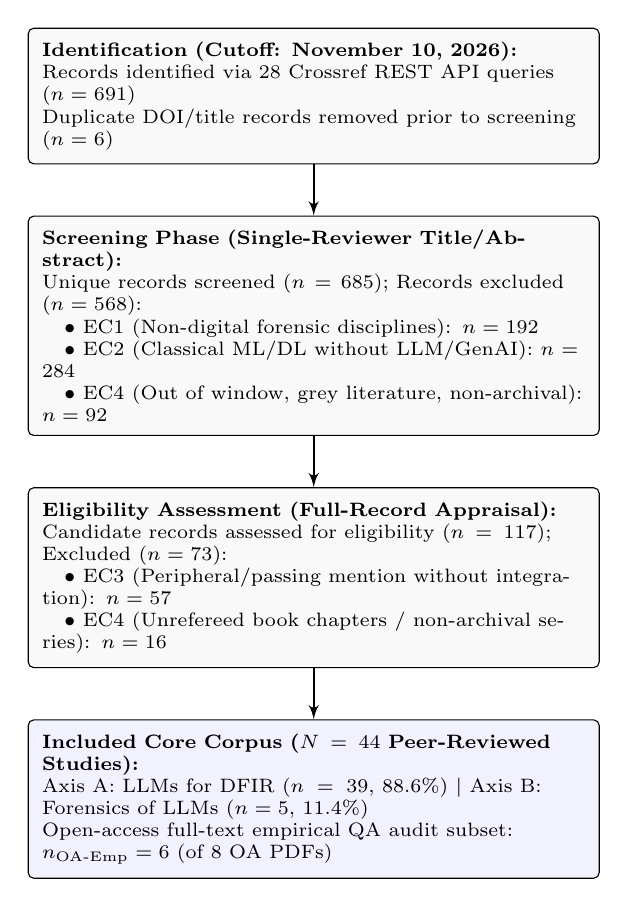
\begin{tikzpicture}[
    node distance=1.0cm and 0.5cm,
    box/.style={draw, rectangle, rounded corners=2pt, text width=6.9cm, align=left, font=\scriptsize, inner sep=5pt, fill=gray!5},
    arr/.style={-latex', thick}
]

\node[box] (id) {\textbf{Identification (Cutoff: November 10, 2026):}\\
Records identified via 28 Crossref REST API queries ($n = 691$)\\
Duplicate DOI/title records removed prior to screening ($n = 6$)};

\node[box, below=0.65cm of id] (screen) {\textbf{Screening Phase (Single-Reviewer Title/Abstract):}\\
Unique records screened ($n = 685$); Records excluded ($n = 568$):\\
\quad $\bullet$ EC1 (Non-digital forensic disciplines): $n = 192$\\
\quad $\bullet$ EC2 (Classical ML/DL without LLM/GenAI): $n = 284$\\
\quad $\bullet$ EC4 (Out of window, grey literature, non-archival): $n = 92$};

\node[box, below=0.65cm of screen] (elig) {\textbf{Eligibility Assessment (Full-Record Appraisal):}\\
Candidate records assessed for eligibility ($n = 117$); Excluded ($n = 73$):\\
\quad $\bullet$ EC3 (Peripheral/passing mention without integration): $n = 57$\\
\quad $\bullet$ EC4 (Unrefereed book chapters / non-archival series): $n = 16$};

\node[box, below=0.65cm of elig, fill=blue!5] (incl) {\textbf{Included Core Corpus ($N = 44$ Peer-Reviewed Studies):}\\
Axis A: LLMs for DFIR ($n=39$, 88.6\%) $\mid$ Axis B: Forensics of LLMs ($n=5$, 11.4\%)\\
Open-access full-text empirical QA audit subset: $n_{\text{OA-Emp}} = 6$ (of 8 OA PDFs)};

\draw[arr] (id) -- (screen);
\draw[arr] (screen) -- (elig);
\draw[arr] (elig) -- (incl);

\end{tikzpicture}
\caption{PRISMA 2020 flow diagram detailing Crossref identification (cutoff November 10, 2026), screening, eligibility, and dual-axis inclusion ($N=44$).}
\label{fig:prisma_flowchart}
\end{figure}


During title and metadata screening of all 685 unique records, 568 entries were excluded: 192 addressed physical or medical forensics (EC1), 284 employed conventional non-LLM classifiers (EC2), and 92 fell outside archival peer-reviewed or temporal criteria (EC4). The remaining 117 candidate records underwent detailed eligibility appraisal, during which 73 publications were excluded: 57 failed EC3 due to incidental mentions without operational forensic integration, and 16 failed EC4 because they originated from unrefereed book chapters or non-archival book series.

Filtering produced a final validated core corpus of $N=44$ peer-reviewed studies (22 journal articles and 22 conference/workshop proceedings). Within this set, two domain-adjacent empirical studies retrieved by the forensic and incident-response queries were deliberately retained and flagged as boundary cases: Farber~\cite{farber2025_scpaiscp}, which evaluates multimodal LLMs on crime-scene photographic triage with ten forensic examiners, and Tian et al.~\cite{tian2026_gala}, which applies graph-augmented LLM agents to microservice incident response. Because this review was conducted by a single human author without a second independent human screener, coding reliability was audited through a deterministic dual-pass verification protocol comparing automated lexical rule classification (executed over titles and the 40 reconstructed abstracts/full texts) against curated manual coding across $N=44$. Observed agreement reached 94.1\% (Cohen's $\kappa=0.821$) on dedicated local-model classification across the 34 empirical DFIR tools (the two rule divergences stemmed from full-text-only model details in~\cite{clark2025_large} and parenthetical wording in~\cite{michelet2024_chatgpt}). All scripts, JSON snapshots, and coding matrices are publicly archived for independent audit (\url{https://github.com/casousavng/llm-digital-forensics-systematic-review}).

\subsection{Quality Appraisal and Open-Access Full-Text Audit}
In accordance with PRISMA 2020 risk-of-bias reporting standards, methodological quality was evaluated against four forensic engineering criteria: \textbf{QA1 (Artifact Provenance)}, specifying evidence source formats, disk/memory structures, or cryptographic baselines; \textbf{QA2 (Reproducibility Manifest)}, disclosing complete inference parameters (system prompt, temperature $T$, top-$p$, random seed, and model/tokenizer versions); \textbf{QA3 (Ground-Truth Objectivity)}, evaluating accuracy against deterministic or labeled ground-truth baselines; and \textbf{QA4 (Robustness and Adversarial Testing)}, quantitatively measuring hallucination rates, context degradation, or evidence-borne prompt injection.

Although OpenAlex enrichment expanded abstract visibility to 90.9\% ($n=40$) of the corpus, publisher paywalls restrict programmatic full-text access for closed-access papers; claiming complete QA1--QA4 scores from abstracts alone would overstate verifiable evidence. Instead, we executed a rigorous, auditable full-text QA1--QA4 inspection across the \textbf{open-access archival full-text subset} available on disk ($n=8$ PDFs, comprising $n_{\text{OA-Emp}}=6$ empirical implementations/datasets and 2 comprehensive surveys~\cite{jelodar2026_large, wickramasekara2025_exploring}), complemented by OpenAlex abstract verification across the remaining 36 studies. Table~\ref{tab:qa_audit} summarizes the exact empirical audit results.

\begin{table}[!t]
\caption{Quantitative Forensic Quality Appraisal (QA1--QA4) Across the Open-Access Empirical Full-Text Audit Subset ($n_{\text{OA-Emp}}=6$)}
\label{tab:qa_audit}
\centering
\scriptsize
\setlength{\tabcolsep}{2pt}
\begin{tabular}{lccccp{1.75cm}}
\toprule
\textbf{Study} & \textbf{QA1} & \textbf{QA2} & \textbf{QA3} & \textbf{QA4} & \textbf{Primary} \\
 & \textbf{Prov.} & \textbf{Manif.} & \textbf{GT} & \textbf{Adv/Hal} & \textbf{Dataset Tier} \\
\midrule
Michelet et al.~\cite{michelet2024_chatgpt} & Yes & No & Yes & Hal. & Fictive Case \\
Chakir et al.~\cite{chakir2025_forensicsdata} & Yes & No & Yes & Hal. & Public (5k QCA) \\
Clark \& Chen~\cite{clark2025_large} & No & Part.* & Yes & Adv. & API Traces \\
Khatiwala et al.~\cite{khatiwala2025_evaluating} & Yes & No & Yes & No & CTF (13~GB) \\
Studiawan et al.~\cite{studiawan2025_towards} & Yes & No & Yes & Hal. & Public Bench. \\
Hammar et al.~\cite{hammar2026_incident} & No & Part.* & Yes & Hal. & Testbed / Synth. \\
\midrule
\textbf{Pass Rate ($n=6$)} & \textbf{4/6} & \textbf{0/6} & \textbf{6/6} & \textbf{5/6} & \textbf{0/6 Prompt Inj.} \\
 & \textbf{(66.7\%)} & \textbf{(0.0\%)} & \textbf{(100\%)} & \textbf{(83.3\%)} & \textbf{Stress-Tested} \\
\bottomrule
\multicolumn{6}{p{7.8cm}}{\tiny *Partial QA2: fixed random seeds disclosed, but complete forensic manifest (weights hash, $T$/top-$p$, runtime flags) omitted.}
\end{tabular}
\end{table}

The quantitative audit exposes an unmistakable structural deficit. While all six audited empirical studies measure performance against labeled ground-truth baselines (QA3: 6/6) and five evaluate or analyze hallucination or adversarial malware behavior (QA4: 5/6), \textbf{none (0/6)} publish a complete forensic reproducibility manifest (QA2), and \textbf{none (0/6)} stress-test evidence-borne indirect prompt injection. Even across the entire $N=44$ corpus, only one dedicated study~\cite{kim2026_evidenceborne} empirically targets evidence-borne prompt injection in forensic triage. Operational prototypes advance rapidly; forensic reproducibility standards lag behind.

\section{Bibliometric Analysis (RQ1)}
\label{sec:bibliometrics}

To address RQ1, this section quantifies publication volume, venue concentration, geographic collaboration, co-authorship topology, and decoupled orthogonal structural trends across the validated core corpus ($N=44$).

\subsection{Temporal Growth and Venue Disaggregation}
Scholarly output linking generative language models and digital forensics exhibits steep, non-linear growth between 2021 and late 2026. No peer-reviewed studies meeting eligibility criteria appeared in 2021 or 2022. Initial domain contributions emerged in 2023 with 3 publications (6.8\%: 2 journal articles and 1 workshop paper), anchored by conceptual analyses evaluating ChatGPT against investigative workflows~\cite{scanlon2023_digital, scanlon2023_chatgpt} and early LLM invocation-log forensics~\cite{chernyshev2023_towards}.

Volume increased modestly in 2024 to 4 papers (9.1\%: 2 journal articles and 2 conference papers), marking the transition toward empirical benchmarks on memory dumps, assisted report drafting, and multi-agent platform artifacts~\cite{oh2024_volgpt, michelet2024_chatgpt, walker2024_forensic}. A sharp inflection occurred during 2025 and 2026. Annual output expanded fourfold to 16 articles in 2025 (36.4\%: 8 journals and 8 proceedings) and reached 21 articles in 2026 year-to-date through November 10, 2026 (47.7\%: 10 journals and 11 proceedings). Together, 2025 and 2026 account for 84.1\% ($n=37$) of the corpus, split evenly across archival journals ($n=22$, 50.0\%) and peer-reviewed proceedings ($n=22$, 50.0\%). Fig.~\ref{fig:temporal_distribution} visualizes this annual trajectory disaggregated by publication type. Because 2026 indexing reflects a partial year, final 2026 volume will almost certainly exceed the observed peak.

\begin{figure}[!t]
\centering
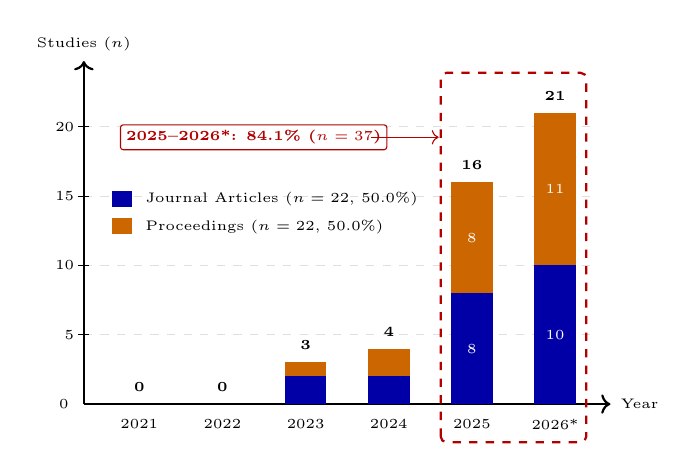
\begin{tikzpicture}[scale=0.88, font=\scriptsize]
  % Axes
  \draw[->, thick] (0,0) -- (7.6,0) node[right, font=\tiny] {Year};
  \draw[->, thick] (0,0) -- (0,4.95) node[above, font=\tiny] {Studies ($n$)};

  % Horizontal gridlines and y-ticks (scale: 1 unit = 5 articles -> y = n/5)
  \foreach \y/\lbl in {1/5, 2/10, 3/15, 4/20} {
    \draw[gray!25, dashed] (0,\y) -- (7.3,\y);
    \draw (-0.08,\y) -- (0.08,\y) node[left=2pt, font=\tiny] {\lbl};
  }
  \node[left=2pt, font=\tiny] at (0,0) {0};

  % Stacked bars: (x, journal_n, proc_n, total_lbl, year_lbl)
  % 2021: 0, 0
  \node[below=2pt, font=\tiny] at (0.8,0) {2021};
  \node[above=1pt, font=\tiny\bfseries] at (0.8,0) {0};

  % 2022: 0, 0
  \node[below=2pt, font=\tiny] at (2.0,0) {2022};
  \node[above=1pt, font=\tiny\bfseries] at (2.0,0) {0};

  % 2023: J=2 (0.4), P=1 (0.2), Total=3 (0.6)
  \fill[blue!65!black] (2.9,0) rectangle (3.5,0.4);
  \fill[orange!80!black] (2.9,0.4) rectangle (3.5,0.6);
  \node[below=2pt, font=\tiny] at (3.2,0) {2023};
  \node[above=1pt, font=\tiny\bfseries] at (3.2,0.6) {3};

  % 2024: J=2 (0.4), P=2 (0.4), Total=4 (0.8)
  \fill[blue!65!black] (4.1,0) rectangle (4.7,0.4);
  \fill[orange!80!black] (4.1,0.4) rectangle (4.7,0.8);
  \node[below=2pt, font=\tiny] at (4.4,0) {2024};
  \node[above=1pt, font=\tiny\bfseries] at (4.4,0.8) {4};

  % 2025: J=8 (1.6), P=8 (1.6), Total=16 (3.2)
  \fill[blue!65!black] (5.3,0) rectangle (5.9,1.6);
  \fill[orange!80!black] (5.3,1.6) rectangle (5.9,3.2);
  \node[white, font=\tiny] at (5.6,0.8) {8};
  \node[white, font=\tiny] at (5.6,2.4) {8};
  \node[below=2pt, font=\tiny] at (5.6,0) {2025};
  \node[above=1pt, font=\tiny\bfseries] at (5.6,3.2) {16};

  % 2026 YTD: J=10 (2.0), P=11 (2.2), Total=21 (4.2)
  \fill[blue!65!black] (6.5,0) rectangle (7.1,2.0);
  \fill[orange!80!black] (6.5,2.0) rectangle (7.1,4.2);
  \node[white, font=\tiny] at (6.8,1.0) {10};
  \node[white, font=\tiny] at (6.8,3.1) {11};
  \node[below=2pt, font=\tiny] at (6.8,0) {2026*};
  \node[above=1pt, font=\tiny\bfseries] at (6.8,4.2) {21};

  % Highlight bracket for 2025-2026 surge
  \draw[red!70!black, thick, dashed, rounded corners=2pt] (5.15,-0.55) rectangle (7.25,4.78);
  \node[fill=white, draw=red!70!black, rounded corners=1pt, font=\tiny\bfseries, text=red!70!black, inner sep=2pt] at (2.45,3.85) {2025--2026*: 84.1\% ($n=37$)};
  \draw[->, red!70!black, thin] (4.15,3.85) -- (5.12,3.85);

  % Legend
  \fill[blue!65!black] (0.4,2.85) rectangle (0.7,3.08);
  \node[right, font=\tiny] at (0.75,2.96) {Journal Articles ($n=22$, 50.0\%)};
  \fill[orange!80!black] (0.4,2.45) rectangle (0.7,2.68);
  \node[right, font=\tiny] at (0.75,2.56) {Proceedings ($n=22$, 50.0\%)};
\end{tikzpicture}
\caption{Annual publication trajectory of the validated corpus ($N=44$) disaggregated by publication venue type. *2026 reflects year-to-date Crossref indexing through November 10, 2026.}
\label{fig:temporal_distribution}
\end{figure}


\subsection{Dissemination Venues and Journal Concentration}
Publication outlets exhibit marked concentration within specialized digital forensics journals alongside selective penetration into flagship computer security conferences. Table~\ref{tab:venue_distribution} reports all recurring venues publishing two or more corpus studies.

\begin{table}[!t]
\caption{Publication Distribution Across Recurring Venues ($N=44$)}
\label{tab:venue_distribution}
\centering
\scriptsize
\begin{tabular}{p{4.8cm}cc}
\toprule
\textbf{Publication Venue} & \textbf{Articles ($n$)} & \textbf{Share (\%)} \\
\midrule
Forensic Science International: Digital Investigation (Elsevier) & 13 & 29.5\% \\
Journal of Forensic Sciences (Wiley) & 3 & 6.8\% \\
IEEE Int. Symp. on Digital Forensics and Security (ISDFS) & 3 & 6.8\% \\
Journal of Cybersecurity, Digital Forensics and Jurisprudence & 2 & 4.5\% \\
IEEE Annual COMPSAC Conference & 2 & 4.5\% \\
Single-Appearance Peer-Reviewed Journals \& Conferences* & 21 & 47.7\% \\
\midrule
\textbf{Total Validated Corpus} & \textbf{44} & \textbf{100.0\%}$^\dagger$ \\
\bottomrule
\multicolumn{3}{p{7.8cm}}{\tiny *Includes flagship venues with $n=1$ each: IEEE S\&P~\cite{xu2026_recovering}, NDSS~\cite{hammar2026_incident}, IEEE TIFS~\cite{zheng2025_avagent}, ACM SIGKDD~\cite{xu2025_enhancing}, ACM CIKM~\cite{xu2024_transforming}, IEEE/ACM ASE~\cite{tian2026_gala}, ACM DTRAP~\cite{michelet2025_finetuning}, and IEEE Access~\cite{kao2026_a}. $^\dagger$Individual rounded shares sum to 99.8\% due to single-decimal rounding.}
\end{tabular}
\end{table}

\textit{Forensic Science International: Digital Investigation} (FSIDI) dominates scholarly dissemination with 13 articles (29.5\%), reflecting strong domain gatekeeping by reviewers familiar with evidentiary reproducibility and custody standards. Specialized forums such as Wiley's \textit{Journal of Forensic Sciences} ($n=3$) and IEEE ISDFS ($n=3$) form a secondary tier. Crucially, the remaining 21 single-appearance outlets (47.7\%) are not peripheral; they include top-tier security and data-mining venues such as the IEEE Symposium on Security and Privacy (IEEE S\&P)~\cite{xu2026_recovering}, NDSS~\cite{hammar2026_incident}, IEEE Transactions on Information Forensics and Security (TIFS)~\cite{zheng2025_avagent}, ACM SIGKDD~\cite{xu2025_enhancing}, and IEEE/ACM ASE~\cite{tian2026_gala}, demonstrating mainstream security-community engagement with forensic LLM problems.

\subsection{Geographic, Institutional, and Citation Distribution}
Cross-validating all 44 DOIs against OpenAlex resolves Crossref's sparse affiliation reporting, raising structured institutional and geographic coverage from 61.4\% ($n=27$) in Crossref to 97.7\% ($n=43$ of 44 studies) in OpenAlex. Across these 43 affiliation-indexed publications, 18 countries are represented (Table~\ref{tab:geo_distribution}). Using full-counting attribution (crediting each participating country once per multi-country paper, totaling 56 country appearances), the United States leads with $n=17$ papers (39.5\% of affiliation-indexed works), followed by South Korea, Switzerland, and Ireland ($n=5$ each, 11.6\% each), Australia and Germany ($n=4$ each, 9.3\% each), and the United Kingdom ($n=3$, 7.0\%). Leading institutional contributors include University College Dublin ($n=5$), Louisiana State University ($n=4$), University of Lausanne ($n=4$), University of Baltimore ($n=3$), and Sungkyunkwan University ($n=3$). Multi-institutional co-authorship appears in 20 of 43 indexed papers (46.5\%), whereas cross-border international collaboration remains confined to 8 papers (18.6\%, e.g.,~\cite{michelet2025_finetuning, hammar2026_a, sava2026_triagecpg}), reflecting divergent statutory evidentiary frameworks across court jurisdictions.

\begin{table}[!t]
\caption{Geographic Distribution and Cross-Database Citation Impact ($n=43$ OpenAlex Affiliation-Indexed Papers; $N=44$ Corpus)}
\label{tab:geo_distribution}
\centering
\scriptsize
\begin{tabular}{p{3.9cm}cc}
\toprule
\textbf{Country / Bibliometric Indicator} & \textbf{Count ($n$)} & \textbf{Share (\%)} \\
\midrule
United States & 17 & 39.5\% \\
South Korea, Switzerland, Ireland & 5 each & 11.6\% each \\
Australia, Germany & 4 each & 9.3\% each \\
United Kingdom & 3 & 7.0\% \\
Turkey, Canada & 2 each & 4.7\% each \\
Other (CN, EG, ID, IN, JP, MA, NL, TW, IL) & 1 each & 2.3\% each \\
\midrule
Multi-Institutional Papers (of $n=43$) & 20 & 46.5\% \\
Cross-Border Collaborations (of $n=43$) & 8 & 18.6\% \\
\midrule
Crossref Citations ($N=44$, Sum / Mean / Med.) & 385 & 8.75 / 2.0 \\
OpenAlex Citations ($N=44$, Sum / Mean / Med.) & 903 & 20.52 / 4.0 \\
Uncited Papers (Crossref / OpenAlex) & 18 / 14 & 40.9\% / 31.8\% \\
\bottomrule
\multicolumn{3}{p{7.8cm}}{\tiny Note: Country counts employ full counting across 8 cross-border papers, yielding 56 country appearances across 43 affiliation-indexed studies (sum of shares exceeds 100\%). Citation triangulation compares Crossref (\texttt{is-referenced-by-count}) against OpenAlex (\texttt{cited\_by\_count}) on November 19, 2026.}
\end{tabular}
\end{table}

Cross-database citation triangulation confirms rapid scholarly uptake despite the recency of the corpus. Crossref records 385 cumulative citations (mean 8.75, median 2.0, maximum 74; 18 uncited [40.9\%]), whereas OpenAlex indexes 903 cumulative citations (mean 20.52, median 4.0, maximum 190; 14 uncited [31.8\%]). Across both indexes, impact concentrates heavily in early roadmaps and pioneer empirical benchmarks (reported as Crossref / OpenAlex citations): Scanlon et al.~\cite{scanlon2023_chatgpt} (74 / 190), Michelet and Breitinger~\cite{michelet2024_chatgpt} (41 / 92), Wickramasekara et al.~\cite{wickramasekara2025_exploring} (28 / 88), Jelodar et al.~\cite{jelodar2026_large} (31 / 81), Sharma et al.~\cite{sharma2025_forensicllm} (26 / 59), and Farber~\cite{farber2025_scpaiscp} (36 / 53).

\subsection{Co-Authorship Networks and Orthogonal Taxonomic Mapping}
Graph reconstruction of Crossref author metadata identifies 155 author appearances across 130 unique researchers (mean 3.52 authors per paper; 40 multi-authored [90.9\%] vs.\ 4 single-authored [9.1\%]). The collaboration network partitions into 30 connected components anchored by three productive clusters: a 13-author U.S.\ memory and agentic-forensics group centered on Baggili ($n=4$) and Gharaibeh ($n=3$)~\cite{sharma2025_forensicllm, gharaibeh2026_rusting, satter2026_with}; a 12-author European cluster linking University College Dublin, University of Lausanne, University of Augsburg, and the Netherlands Forensic Institute led by Scanlon ($n=6$) and Breitinger ($n=5$)~\cite{scanlon2023_digital, michelet2025_finetuning, studiawan2025_towards}; and a 9-author Baltimore/Towson group led by Xu ($n=3$)~\cite{xu2024_transforming, zhou2025_forensic, khatiwala2025_evaluating}.

To avoid conflating mutually exclusive themes with orthogonal architectural attributes, we code all 44 studies along two separated layers depicted in Fig.~\ref{fig:subdomain_matrix}. First, mutually exclusive thematic clustering partitions the corpus into six operational subdomains summing exactly to $N=44$: \textit{Evidence Triage, Reporting, and Datasets} leads with 40.9\% ($n=18$), covering report drafting, keyword expansion, graph extraction, multilingual chat triage, and dataset construction~\cite{michelet2024_chatgpt, chakir2025_forensicsdata, yoo2026_scpllmscp, johnson2026_aiassisted}; \textit{Incident Response, Logs, and Agentic SOC} accounts for 20.5\% ($n=9$), addressing multi-agent correlation, cloud log parsing, timeline evaluation, and response planning~\cite{liu2025_autobnb, hammar2026_incident, alharthi2025_llmpowered, studiawan2025_towards}; \textit{Malware Analysis and Reverse Engineering} represents 13.6\% ($n=6$), spanning behavioral system-call classification, Code Property Graphs, and APK analysis~\cite{clark2025_large, sava2026_triagecpg, zheng2025_avagent, ozyurt2026_llmorchestrated}; \textit{Forensics of LLM and Agentic Systems} captures 11.4\% ($n=5$), examining artifact recovery from AutoGen, MCP memory, mobile local LLMs, invocation logs, and AI investigative readiness~\cite{chernyshev2023_towards, walker2024_forensic, xu2026_recovering, satter2026_with, scanlon2026_investigation}; \textit{Volatile Memory Forensics (LLM-Assisted)} accounts for 6.8\% ($n=3$), focusing on ransomware RAM triage, Volatility migration, and privacy-preserving wallet memory analysis~\cite{oh2024_volgpt, gharaibeh2026_rusting, kao2026_a}; and \textit{Legal Admissibility, Explainability, and Covert Artifacts} accounts for 6.8\% ($n=3$), examining premise-acceptance bias, offline neuro-symbolic explainability, and LSB steganography~\cite{trivedi2026_when, tiwari2026_xforensicnet, sudheer2026_least}.

\begin{figure}[!t]
\centering
\resizebox{\columnwidth}{!}{%
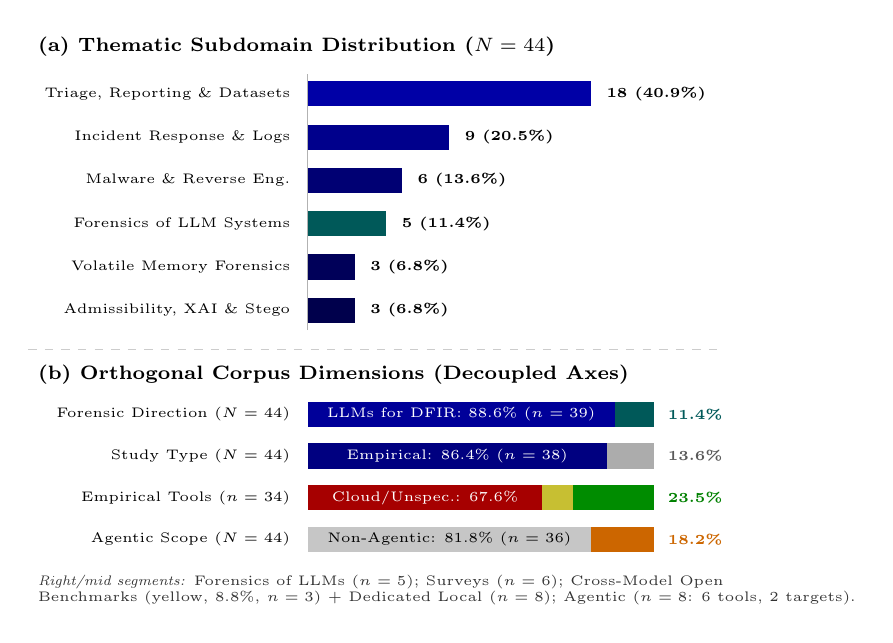
\begin{tikzpicture}[font=\scriptsize]
  % Panel A: Six Operational Subdomains (N=44)
  \node[anchor=west, font=\scriptsize\bfseries] at (0,5.25) {(a) Thematic Subdomain Distribution ($N=44$)};

  % Scale: 18 studies = 3.6 cm -> x = n * 0.20
  \foreach \y/\lbl/\n/\pct/\col in {
    4.65/{Triage, Reporting \& Datasets}/18/{40.9\%}/blue!65!black,
    4.10/{Incident Response \& Logs}/9/{20.5\%}/blue!55!black,
    3.55/{Malware \& Reverse Eng.}/6/{13.6\%}/blue!45!black,
    3.00/{Forensics of LLM Systems}/5/{11.4\%}/teal!70!black,
    2.45/{Volatile Memory Forensics}/3/{6.8\%}/blue!35!black,
    1.90/{Admissibility, XAI \& Stego}/3/{6.8\%}/blue!30!black%
  } {
    \node[anchor=east, font=\tiny] at (3.45,\y) {\lbl};
    \fill[\col] (3.55,\y-0.16) rectangle ({3.55+\n*0.20},\y+0.16);
    \node[anchor=west, font=\tiny\bfseries] at ({3.62+\n*0.20},\y) {\n\ (\pct)};
  }
  \draw[gray!60] (3.55,1.65) -- (3.55,4.90);

  % Divider
  \draw[gray!40, dashed] (0,1.40) -- (8.85,1.40);

  % Panel B: Orthogonal Structural Indicators (100% stacked horizontal bars, width = 4.4cm)
  \node[anchor=west, font=\scriptsize\bfseries] at (0,1.08) {(b) Orthogonal Corpus Dimensions (Decoupled Axes)};

  % Row 1: Forensic Direction (N=44): 39 (88.6%) vs 5 (11.4%)
  \node[anchor=east, font=\tiny] at (3.45,0.58) {Forensic Direction ($N=44$)};
  \fill[blue!60!black] (3.55,0.42) rectangle ({3.55+4.4*0.886},0.74);
  \fill[teal!70!black] ({3.55+4.4*0.886},0.42) rectangle ({3.55+4.4},0.74);
  \node[white, font=\tiny] at (5.50,0.58) {LLMs for DFIR: 88.6\% ($n=39$)};
  \node[anchor=west, font=\tiny\bfseries, text=teal!70!black] at (8.00,0.58) {11.4\%};

  % Row 2: Study Type (N=44): 38 (86.4%) vs 6 (13.6%)
  \node[anchor=east, font=\tiny] at (3.45,0.05) {Study Type ($N=44$)};
  \fill[blue!50!black] (3.55,-0.11) rectangle ({3.55+4.4*0.864},0.21);
  \fill[gray!65] ({3.55+4.4*0.864},-0.11) rectangle ({3.55+4.4},0.21);
  \node[white, font=\tiny] at (5.45,0.05) {Empirical: 86.4\% ($n=38$)};
  \node[anchor=west, font=\tiny\bfseries, text=gray!70!black] at (8.00,0.05) {13.6\%};

  % Row 3: Empirical DFIR Tools (n=34): Cloud/Unspec 23 (67.6%) + Cross-Model Open 3 (8.8%) + Dedicated Local 8 (23.5%)
  \node[anchor=east, font=\tiny] at (3.45,-0.48) {Empirical Tools ($n=34$)};
  \fill[red!65!black] (3.55,-0.64) rectangle ({3.55+4.4*0.676},-0.32);
  \fill[yellow!75!black] ({3.55+4.4*0.676},-0.64) rectangle ({3.55+4.4*0.765},-0.32);
  \fill[green!55!black] ({3.55+4.4*0.765},-0.64) rectangle ({3.55+4.4},-0.32);
  \node[white, font=\tiny] at (5.04,-0.48) {Cloud/Unspec.: 67.6\%};
  \node[anchor=west, font=\tiny\bfseries, text=green!50!black] at (8.00,-0.48) {23.5\%};

  % Row 4: Orchestration (N=44): Non-Agentic 36 (81.8%) vs Agentic 8 (18.2%)
  \node[anchor=east, font=\tiny] at (3.45,-1.01) {Agentic Scope ($N=44$)};
  \fill[gray!45] (3.55,-1.17) rectangle ({3.55+4.4*0.818},-0.85);
  \fill[orange!80!black] ({3.55+4.4*0.818},-1.17) rectangle ({3.55+4.4},-0.85);
  \node[black, font=\tiny] at (5.35,-1.01) {Non-Agentic: 81.8\% ($n=36$)};
  \node[anchor=west, font=\tiny\bfseries, text=orange!80!black] at (8.00,-1.01) {18.2\%};

  % Compact two-line legend for right-hand & middle segments
  \node[anchor=west, font=\tiny, text=black!80, align=left] at (0,-1.65) {\textit{Right/mid segments:} Forensics of LLMs ($n=5$); Surveys ($n=6$); Cross-Model Open\\Benchmarks (yellow, 8.8\%, $n=3$) + Dedicated Local ($n=8$); Agentic ($n=8$: 6 tools, 2 targets).};
\end{tikzpicture}%
}
\caption{Thematic subdomain ranking and decoupled orthogonal structural indicators across the validated corpus ($N=44$), verified via Crossref and OpenAlex (40/44 abstracts/full texts). Deployment locality is evaluated strictly over empirical LLM-for-DFIR tool studies ($n=34$).}
\label{fig:subdomain_matrix}
\end{figure}


Second, decoupled orthogonal coding separates four independent structural dimensions across the corpus. Along the \textit{Forensic Direction} axis, 88.6\% ($n=39$) apply LLMs as DFIR instruments whereas 11.4\% ($n=5$) examine LLM platforms as forensic subjects. Along the \textit{Study Type} axis, 86.4\% ($n=38$) present empirical implementations, benchmarks, datasets, or artifact studies, whereas 13.6\% ($n=6$) are conceptual roadmaps, surveys, or readiness reviews~\cite{scanlon2023_digital, scanlon2023_chatgpt, wickramasekara2025_exploring, chernyshev2026_large, jelodar2026_large, scanlon2026_investigation}. Measuring \textit{Deployment Locality} strictly over the $n=34$ empirical LLM-for-DFIR tool studies (excluding six surveys and four empirical LLM-as-subject studies to avoid denominator inflation, verified across 40/44 abstracts and full texts) reveals three distinct tiers: only 23.5\% ($n=8$) design, fine-tune, or deploy dedicated local, offline, or lightweight open-weights models~\cite{sharma2025_forensicllm, michelet2024_chatgpt, michelet2025_finetuning, tiwari2026_xforensicnet, kao2026_a, hammar2026_incident, hammar2026_a, clark2025_large}, another 8.8\% ($n=3$) include open-weights baselines within multi-model comparative benchmarks~\cite{chakir2025_forensicsdata, studiawan2025_towards, sava2026_triagecpg}, and the remaining 67.6\% ($n=23$) rely on commercial cloud APIs or omit explicit local air-gapped deployment guarantees. Independently, along the \textit{Agentic Orchestration} axis, 18.2\% ($n=8$) of the corpus engages agentic architectures: 13.6\% ($n=6$) implement multi-agent DFIR or malware pipelines~\cite{liu2025_autobnb, ozyurt2026_llmorchestrated, zgzler2026_eventdriven, tian2026_gala, zheng2025_avagent, tiwari2026_xforensicnet}, and 4.5\% ($n=2$) perform forensic artifact recovery on agentic frameworks~\cite{walker2024_forensic, satter2026_with}.

To verify structural robustness against inclusion-boundary choices, we performed a formal sensitivity analysis excluding all five borderline records simultaneously: the two domain-adjacent studies~\cite{farber2025_scpaiscp, tian2026_gala} and the three short archival papers under four pages~\cite{xu2025_enhancing, sudheer2026_least, hammar2026_a} (including the companion NOMS demo to~\cite{hammar2026_incident}). Across the resulting strict subset ($N_{\text{sens}}=39$, with $n_{\text{emp}}=29$ empirical LLM-for-DFIR tools), the 2025--2026 YTD surge shifts marginally from 84.1\% to 82.1\% ($32/39$), dedicated local/offline tool adoption shifts from 23.5\% to 24.1\% ($7/29$), and cloud/unspecified reliance shifts from 67.6\% to 65.5\% ($19/29$). Every central bibliometric and architectural conclusion remains invariant within 2.1 percentage points. The complete study-by-study coding matrix is tabulated in the Appendix (Table~\ref{tab:master_corpus}).

\subsection{Evaluation Rigor and Benchmark Ground-Truth Audit}
Validating forensic AI claims requires realistic, noise-polluted ground-truth corpora reflecting operational casework rather than clean conversational prompts. Auditing dataset provenance across the open-access empirical subset (Table~\ref{tab:qa_audit}) alongside verifiable dataset disclosures in the broader corpus reveals three distinct empirical tiers. At the lowest external-validity tier, numerous evaluations depend on synthetic logs, fictive mini-cases, or isolated lab scenarios lacking concurrent background noise and corrupted filesystem metadata; within our six audited open-access empirical PDFs, Michelet and Breitinger~\cite{michelet2024_chatgpt} rely on a fictive DFRWS-reviewed case and Hammar et al.~\cite{hammar2026_incident} combine testbed telemetry with LLM-expanded synthetic incident data. At the intermediate tier, closed institutional or law-enforcement casework (e.g.,~\cite{kim2025_digital, ko2026_humansupervised}) offers operational realism but remains sealed under statutory privacy restrictions, precluding independent scientific replication. At the highest reproducibility tier, standardized public corpora remain comparatively scarce: among our six audited full texts, Chakir and Lahsen-Cherif~\cite{chakir2025_forensicsdata} contribute over 5,000 Question-Context-Answer triplets sourced from real malware reports, Khatiwala et al.~\cite{khatiwala2025_evaluating} evaluate a public 13~GB Capture-the-Flag disk image (61 applications, 2,864 databases, 5,870 tables), and Studiawan et al.~\cite{studiawan2025_towards} introduce a standardized timeline evaluation dataset modeled on the NIST Computer Forensics Tool Testing (CFTT) program~\cite{nist_cftt}. Conversely, direct benchmarking against established NIST Computer Forensic Reference Data Sets (CFReDS)~\cite{nist_cfreds} remains conspicuously rare across the corpus. High precision on clean synthetic excerpts therefore provides no guarantee against retrieval collapse on unfiltered, multi-terabyte enterprise images.

\section{Operational Forensic Applications and Targets (RQ2)}
\label{sec:use_cases}

To answer RQ2, this section synthesizes empirical implementations across all six subdomains of the core corpus ($N=44$). Rather than operating as universal autonomous investigators, language models cluster around five DFIR operational bottlenecks (evidence triage and reporting, incident response and log correlation, malware analysis, volatile memory forensics, and covert artifact inspection) alongside a rapidly expanding inverse discipline: digital forensics \textit{of} LLM and agentic systems themselves.

\subsection{Evidence Triage, Reporting, and Benchmark Datasets}
Investigative triage, reporting, and dataset construction represent the largest operational cluster, accounting for 40.9\% ($n=18$) of the validated corpus. Examiners devote substantial effort to synthesizing fragmented artifacts into structured judicial documentation. Michelet and Breitinger~\cite{michelet2024_chatgpt} conducted a foundational experiment examining canonical forensic report structures and benchmarking ChatGPT (GPT-3.5) against a local open-weights baseline (Llama-2-13B) for assisted report drafting. Their evaluation showed that models compress multi-source case details into readable drafts, yet both commercial and local architectures exhibited non-negligible hallucinations and factual inaccuracies unsuitable for unverified court submission.

Subsequent engineering prioritized domain-specific adaptation and on-premise execution. Sharma et al.~\cite{sharma2025_forensicllm} introduced ForensicLLM, a 4-bit quantized LLaMA-3.1-8B architecture fine-tuned on digital forensics Q\&A samples so seized evidentiary material never traverses external networks. Michelet et al.~\cite{michelet2025_finetuning} formalized practical recommendations for instruction-tuning LLMs on forensic tasks, demonstrating through a chat summarization case study that domain fine-tuning improves structured extraction reliability over generic zero-shot prompting.

Complementary architectures couple language models with formal knowledge graphs or human-in-the-loop verification to anchor semantic outputs. Zhou et al.~\cite{zhou2025_forensic} proposed Forensic Intelligence Graphs to extract structured entity relationships from heterogeneous digital evidence, while Khatiwala et al.~\cite{khatiwala2025_evaluating} integrated LLM-refined artifact extraction with a Digital Forensic Knowledge Graph (DFKG), validating artifact traceability on a 13~GB Capture-the-Flag forensic disk image comprising 61 applications, 2,864 databases, and 5,870 tables. At the evidence-intake layer, Yoo and Jeong~\cite{yoo2026_scpllmscp} applied LLM keyword augmentation to improve title-driven file selection, Johnson et al.~\cite{johnson2026_aiassisted} evaluated multilingual online gaming chat triage, and Ko et al.~\cite{ko2026_humansupervised} validated human-supervised multi-model identifier extraction (Claude Sonnet 4.5, GPT-5.2, Gemini 3 Pro) across 273 California DFPI cryptocurrency-fraud ("pig butchering") complaints against dual-rater ground truth ($\kappa=0.969\text{--}0.988$), achieving $F_1=1.000$ on wallet addresses, $F_1=0.911\text{--}0.918$ on URLs, and $F_1=0.865\text{--}0.904$ on loss amounts (vs.\ $F_1 \le 0.381$ for regex/spaCy) while routing 31.1\% ($82/264$) of actionable cases to prioritized human review. In a domain-adjacent pilot study spanning photographic crime-scene triage, Farber~\cite{farber2025_scpaiscp} evaluated GPT-4, Claude, and Gemini across 30 crime-scene images scored by 10 forensic experts, concluding that frontier models serve strictly as preliminary screening aids rather than autonomous analysts. To establish reproducible triage evaluation, Chakir and Lahsen-Cherif~\cite{chakir2025_forensicsdata} introduced ForensicsData, a public benchmark containing over 5,000 Question-Context-Answer triplets derived from real malware analysis reports, while empirical law-enforcement case studies~\cite{kim2025_digital} and early exploratory frameworks~\cite{xu2024_transforming, xu2025_enhancing, wickramasekara2025_exploring} document practical integration barriers.

\subsection{Incident Response, Logs, and Agentic SOC Orchestration}
Incident response, log interpretation, and Security Operations Center (SOC) orchestration constitute 20.5\% ($n=9$) of the corpus. Enterprise intrusions generate high-velocity telemetry across Windows Event Logs, cloud audit trails, and network sensors that overwhelm manual correlation.

Recent studies shift from monolithic single-prompt scripts toward modular agentic orchestration and specialized lightweight models. Liu~\cite{liu2025_autobnb} proposed AutoBnB, a multi-agent incident response architecture partitioning log triage, analysis, and containment reasoning across specialized LLM roles. Similarly, {\"O}zg{\"o}zler et al.~\cite{zgzler2026_eventdriven} designed an Event-Driven Agentic SOC (ED-ASOC) combining supervisor-coordinated LLM agents with SOAR workflows, while Matsuda et al.~\cite{matsuda2025_enhancing} integrated Sigma detection rules, Model Context Protocol interfaces, and operational policies into LLM-assisted response. In cloud environments, Alharthi and Yasaei~\cite{alharthi2025_llmpowered} automated cloud forensic log investigation, and George et al.~\cite{george2025_llm} fused Cyber Threat Intelligence (CTI) knowledge graphs with LLMs to map observed telemetry onto adversary tactics. Extending agentic root-cause analysis to adjacent distributed software operations, Tian et al.~\cite{tian2026_gala} introduced GALA, combining graph-augmented agents for microservice incident triage.

Addressing hallucination and inference cost directly, Hammar et al.~\cite{hammar2026_incident, hammar2026_a} developed fine-tuned lightweight LLM decision-support systems for incident response planning evaluated across testbed and synthetic attack scenarios, demonstrating reduced hallucination rates compared to unconstrained frontier prompting. For forensic timeline evaluation specifically, Studiawan et al.~\cite{studiawan2025_towards} designed a standardized quantitative methodology and dataset modeled on the NIST CFTT framework~\cite{nist_cftt}.

A critical failure mode in automated log and timeline synthesis is narrative coherence bias. Autoregressive models optimize token fluency, compelling disparate log records into a smooth causal storyline. When raw timelines exhibit clock skew, NTP drift, or deliberate anti-forensic timestomping (such as discrepancies between NTFS \texttt{\$STANDARD\_INFORMATION} and \texttt{\$FILE\_NAME} timestamps), unconstrained language models silently smooth away anomalies. Chronological smoothing destroys dispositive evidence. Sound forensic engineering therefore requires deterministic engines such as \texttt{plaso} or \texttt{log2timeline} to fix immutable UTC event sequences before any LLM performs semantic annotation.

\subsection{Malware Analysis and Reverse Engineering}
Malware triage and reverse engineering represent 13.6\% ($n=6$) of the corpus. Modern malicious binaries evade static signature matching via packing, polymorphism, and obfuscated control flow.

Empirical evaluations demonstrate complementary language-model paradigms across behavioral and static layers. Clark and Chen~\cite{clark2025_large} fine-tuned a pretrained RoBERTa transformer on structured Windows application-layer API and system-call traces, capturing behavioral semantics between benign and malicious execution; their 512-token \texttt{prob\_mean} aggregation configuration achieved 92\% recall and an $F_1$ score of 0.94 at the application level. Complementing behavioral analysis, Meskova et al.~\cite{meskova2026_aidriven} applied transformer detection to real-time malware threat analysis, while Jelodar et al.~\cite{jelodar2026_large} synthesized broader LLM capabilities across source-code inspection, vulnerability analysis, and reverse engineering.

To overcome context-window limits on large binaries, recent architectures fuse LLMs with structural program graphs or multi-agent decomposition. Sava et al.~\cite{sava2026_triagecpg} introduced TRIAGE-CPG, pairing Code Property Graphs (CPGs) with eight closed-source and open-weight models evaluated across 1,000 Windows PE binaries (600-sample test split); inspecting roughly 40 of a mean 1,000 functions per binary, the top model reached 0.805 strict balanced accuracy and 0.855 triage balanced accuracy (flagging 65\% of malware, escalating 12\%, and clearing 94\% of benign binaries). Zheng et al.~\cite{zheng2025_avagent} developed AV-Agent, a bottom-up interpretable malware classifier producing auditable attribution chains, and Ozyurt et al.~\cite{ozyurt2026_llmorchestrated} orchestrated parallel three-agent Android APK inspection combining Gemini 2.5 Flash, DeepSeek V3, and GPT-4.1-mini via majority vote.

\subsection{Volatile Memory Forensics (LLM-Assisted)}
LLM-assisted volatile memory forensics accounts for 6.8\% ($n=3$) of the corpus (distinct from memory acquisition \textit{of} LLM applications discussed below). Interpreting raw RAM dumps via Volatility~\cite{case2014volatility} requires deep kernel expertise to separate injected code, unlinked libraries, and hidden network sockets from benign OS state.

Oh et al.~\cite{oh2024_volgpt} introduced volGPT, automating ransomware process triage from structured Volatility outputs to detect process masquerading and volatile artifacts at substantially lower triage latency than manual inspection. Addressing analyzer performance and memory safety, Gharaibeh and Baggili~\cite{gharaibeh2026_rusting} conducted an empirical LLM-assisted migration of 38 Volatility3 Linux plugins from Python to Rust (29,028 lines of code over 68 hours, consuming 900 million tokens at \$2,962); the Rust port achieved a 2.50$\times$ median speedup (up to 210$\times$ on structure traversal), completed 417/417 executions (vs.\ 11.3\% Python runtime failures), and matched canonical output hashes across 68.9\% of comparable runs. Targeting financial privacy in RAM examinations, Kao et al.~\cite{kao2026_a} proposed a local hierarchical LLaMA-3.1-8B Tri-Layer RAG-Decider framework for privacy-preserving cryptocurrency-wallet memory forensics, achieving a 0.84 BERT $F_1$ score across 100 wallet-forensics queries and performing within 0.3\% of commercial ChatGPT-4o overall while surpassing it on reasoning.

\subsection{Digital Forensics of LLM and Agentic Systems}
A rapidly emerging inverse discipline, accounting for 11.4\% ($n=5$) of the corpus, treats LLM runtimes and agentic frameworks not as analytical tools, but as investigative targets generating novel digital evidence. As local inference engines and autonomous agents execute code, browse files, and invoke tools on suspect endpoints, examiners must recover what prompts were issued and which actions executed.

Chernyshev et al.~\cite{chernyshev2023_towards} initiated this axis by analyzing LLM invocation logs to establish forensic traceability of model usage. Walker et al.~\cite{walker2024_forensic} systematically cataloged persistent disk and execution artifacts generated by Microsoft's multi-agent AutoGen platform. At the volatile memory layer, Xu et al.~\cite{xu2026_recovering} demonstrated at IEEE S\&P that conversational histories and cached inference contexts from local mobile LLMs can be recovered and rehosted directly from smartphone RAM dumps. Similarly, Satter et al.~\cite{satter2026_with} demonstrated memory forensic reconstruction of Model Context Protocol (MCP) activity in agentic LLM systems even when application logging is disabled or absent. Synthesizing this emerging domain, Scanlon~\cite{scanlon2026_investigation} formalized digital forensic readiness, evidentiary artifact challenges, and regulatory gaps when investigating proprietary and local AI systems.

\subsection{Admissibility, Explainability, and Covert Artifacts}
The remaining 6.8\% ($n=3$) of the corpus directly targets judicial admissibility, neuro-symbolic explainability, and covert binary artifacts. Trivedi~\cite{trivedi2026_when} empirically tested examiner bias, prompt framing, and evidentiary admissibility across 2,700 trials (analyzed in depth in Section~\ref{sec:custody_crypto}). Tiwari and Nene~\cite{tiwari2026_xforensicnet} introduced X-ForensicNet, a fully offline multi-agent Windows forensics framework coupling local LLM inference, RAG, and neuro-symbolic validation, reporting a 2.8$\times$ investigative speedup and 96.3\% accuracy with explainable reasoning trails. Beyond textual artifacts, Sudheer et al.~\cite{sudheer2026_least} explored LLM-assisted detection and contextual analysis of Least Significant Bit (LSB) image steganography, showing that while generative models cannot replace statistical steganalysis detectors, they assist analysts in triaging extracted covert payloads.

Table~\ref{tab:taxonomy_summary} synthesizes all six operational subdomains, highlighting verified exemplar studies, dominant architectures, and primary forensic safeguards.

\begin{table*}[!t]
\caption{Taxonomic Synthesis of Core Literature Across All Six Mutually Exclusive Subdomains ($N=44$)}
\label{tab:taxonomy_summary}
\centering
\scriptsize
\setlength{\tabcolsep}{3pt}
\begin{tabular}{p{2.2cm}cp{3.7cm}p{2.1cm}cp{3.9cm}}
\toprule
\textbf{Subdomain} & \textbf{Corpus} & \textbf{Verified Exemplar Studies} & \textbf{Dominant Paradigm} & \textbf{RQs} & \textbf{Forensic Relevance \& Safeguards} \\
\midrule
Evidence Triage, Reporting \& Datasets & 18 (40.9\%) & ForensicLLM~\cite{sharma2025_forensicllm}, Reporting~\cite{michelet2024_chatgpt}, DFKG~\cite{khatiwala2025_evaluating}, ForensicsData~\cite{chakir2025_forensicsdata} & Cloud APIs / Local Fine-Tuned & RQ2, RQ3, RQ4 & Case-note synthesis, graph grounding, and benchmark corpora; requires air-gapped local weights and prompt-injection defense. \\
\addlinespace
Incident Response, Logs \& Agentic SOC & 9 (20.5\%) & AutoBnB~\cite{liu2025_autobnb}, Lightweight IR~\cite{hammar2026_incident}, Cloud Logs~\cite{alharthi2025_llmpowered}, Timelines~\cite{studiawan2025_towards} & Multi-Agent / Lightweight LLMs & RQ2, RQ4 & Distributed telemetry correlation and response planning; requires immutable \texttt{plaso} timelines to block narrative smoothing. \\
\addlinespace
Malware Analysis \& Reverse Eng. & 6 (13.6\%) & RoBERTa API Calls~\cite{clark2025_large}, TRIAGE-CPG~\cite{sava2026_triagecpg}, AV-Agent~\cite{zheng2025_avagent}, APK Agents~\cite{ozyurt2026_llmorchestrated} & Fine-Tuned / Graph + Agentic & RQ2, RQ4 & System-call classification and CPG triage; vulnerable to adversarial call/code perturbation and obfuscation. \\
\addlinespace
Forensics of LLM \& Agentic Systems & 5 (11.4\%) & AutoGen~\cite{walker2024_forensic}, Mobile RAM~\cite{xu2026_recovering}, MCP Memory~\cite{satter2026_with}, AI Readiness~\cite{scanlon2026_investigation} & Target Subject (Disk / RAM / Logs) & RQ1, RQ2, RQ3 & Recovers prompts, tool invocations, and KV/context buffers from suspect LLM runtimes under ISO/IEC 27037/27042. \\
\addlinespace
Volatile Memory Forensics (Assisted) & 3 (6.8\%) & volGPT~\cite{oh2024_volgpt}, Rusting Volatility~\cite{gharaibeh2026_rusting}, Wallet RAM~\cite{kao2026_a} & Local / Cloud + Volatility & RQ2, RQ3 & Ransomware triage, Rust plugin migration, and privacy-preserving wallet memory analysis; mandates isolated RAM scratch. \\
\addlinespace
Admissibility, XAI \& Covert Artifacts & 3 (6.8\%) & Premise Bias~\cite{trivedi2026_when}, X-ForensicNet~\cite{tiwari2026_xforensicnet}, LSB Stego~\cite{sudheer2026_least} & Offline Neuro-Symbolic / Audit & RQ3, RQ4 & FRE 702(d) premise auditing, deterministic neuro-symbolic grounding, and covert payload triage. \\
\midrule
\textbf{Total Corpus} & \textbf{44 (100.0\%)} & \multicolumn{4}{p{10.8cm}}{\textit{Mutually exclusive partition across Axis A ($n=39$, LLMs for DFIR) and Axis B ($n=5$, Forensics of LLM Systems).}} \\
\bottomrule
\end{tabular}
\end{table*}


\section{Chain of Custody, Cryptography and Verifiability (RQ3)}
\label{sec:custody_crypto}

To resolve RQ3, this section examines how digital forensics reconciles probabilistic neural inference with statutory custody, deterministic replay, examiner impartiality, and multi-jurisdictional data protection mandates.

\subsection{Normative Alignment and Cryptographic Provenance}
End-to-end digital evidence integrity spans three complementary international standards: ISO/IEC 27037~\cite{iso27037_2012} governs identification, collection, acquisition, and preservation; ISO/IEC 27041~\cite{iso27041_2015} defines assurance criteria for validating investigative methods; and ISO/IEC 27042~\cite{iso27042_2015} establishes procedural guidelines for the analysis and interpretation phase where language models operate, complemented by NIST SP 800-86~\cite{nist_sp800_86}. In conventional forensics, integrity relies on computing cryptographic digests (SHA-256 or BLAKE3) immediately upon disk imaging or memory capture. Any bit-level alteration invalidates the evidentiary baseline.

Introducing generative inference into the analysis phase threatens this continuous audit trail whenever model queries execute as ephemeral, unlogged interactions. Defensible forensic engineering therefore requires treating every inference call as an auditable, cryptographically sealed transaction~\cite{sharma2025_forensicllm, chernyshev2026_large, tiwari2026_xforensicnet}. Specifically, the system prompt, serialized evidence slice, model checkpoint digest, quantization specification, decoding configuration, and raw generated output tokens must be hashed and chained into an append-only provenance ledger signed by the forensic workstation. Should opposing counsel challenge an automated triage note, an independent auditor can verify that the exact evidence slice and model artifact existed unaltered at the recorded timestamp.

\subsection{Inference Determinism, Daubert, and FRE 702(d)}
In common-law jurisdictions governed by the Daubert standard~\cite{daubert1993} and Federal Rule of Evidence 702 (as amended in 2023)~\cite{fre702_2023}, scientific expert methodology is screened for empirical testability, peer review, known or potential error rates, general acceptance (echoing Frye~\cite{frye1923}), and reliable application of principles to case-specific facts under Rule 702(d). Reproducibility failures have already surfaced in litigation: as documented by Trivedi~\cite{trivedi2026_when}, in \textit{Matter of Weber} (2024) a surrogate's court submitted the same Microsoft Copilot query across three computers and obtained three divergent figures, while the testifying expert could not recall the exact prompt used.

Practitioners frequently assume that setting greedy decoding temperature to zero ($T=0.0$) guarantees exact bitwise replay. Hardware execution physics refutes this assumption~\cite{michelet2024_chatgpt, trivedi2026_when, scanlon2026_investigation}. Modern GPU tensor libraries (such as NVIDIA cuBLAS and cuDNN) execute parallel warp reductions whose floating-point summation order varies dynamically with thread scheduling and batch composition. Because IEEE 754 floating-point addition in FP16, BF16, and FP32 is non-associative, microscopic rounding variations ($\approx 10^{-6}$) alter least significant mantissa bits in logit vectors. Whenever two candidate vocabulary tokens exhibit near-identical logits, thread-scheduling jitter flips the greedy $\arg\max$ selection; once an alternate token enters the autoregressive context window, subsequent text diverges rapidly. Deterministic replay remains unattainable on standard batched GPU pipelines.

To establish auditable execution verifiability under ISO/IEC 27041 and FRE 702, forensic architectures require a complete cryptographic execution manifest $\mathcal{M}$:
\begin{align}
\label{eq:forensic_manifest}
\mathcal{M} = \langle &\mathcal{H}_{\text{weights}}, \mathcal{H}_{\text{vocab}}, \mathcal{H}_{\text{tmpl}}, \mathcal{H}_{\text{prompt}}, \mathcal{H}_{\text{evidence}}, \nonumber \\
&q_{\text{quant}}, \theta_{\text{dec}}, \sigma_{\text{seed}}, \phi_{\text{runtime}}, \kappa_{\text{det}} \rangle
\end{align}
Here, $\mathcal{H}_{\text{weights}}$, $\mathcal{H}_{\text{vocab}}$, $\mathcal{H}_{\text{tmpl}}$, $\mathcal{H}_{\text{prompt}}$, and $\mathcal{H}_{\text{evidence}}$ denote immutable SHA-256 digests of the model checkpoint, tokenizer vocabulary, chat template, system/user prompt, and input evidence chunk; $q_{\text{quant}}$ records the exact quantization format (e.g., GGUF $Q4\_K\_M$ or FP16); $\theta_{\text{dec}} = (T, \text{top-}p, \text{top-}k, \text{rep\_pen})$ fixes all decoding hyperparameters; $\sigma_{\text{seed}}$ pins the pseudo-random seed; $\phi_{\text{runtime}}$ logs exact engine, compiler, and driver versions; and $\kappa_{\text{det}}$ enforces runtime-specific determinism controls (e.g., \texttt{CUBLAS\_WORKSPACE\_CONFIG=:4096:8} and \texttt{torch.use\_deterministic\_algorithms(True)} for PyTorch/vLLM backends, or fixed single-sequence batch size, deterministic thread affinity, and \texttt{--temp 0 --seed} pinning for \texttt{llama.cpp}/GGML engines). Single-threaded CPU execution eliminates GPU warp non-determinism entirely, yet its low token throughput renders it operationally impractical for bulk multi-terabyte triage; instead, laboratories should combine batched local GPU triage with targeted deterministic CPU verification strictly on short, dispositive evidence excerpts selected for courtroom presentation.

Table~\ref{tab:daubert_mapping} maps Daubert and FRE 702 admissibility pillars directly against LLM technical constraints and concrete engineering safeguards.

\begin{table*}[!t]
\caption{Admissibility Assessment: Daubert Standard and FRE 702(d) Criteria vs. Large Language Model Realities in Digital Forensics}
\label{tab:daubert_mapping}
\centering
\scriptsize
\begin{tabular}{p{2.6cm}p{4.2cm}p{4.4cm}p{4.4cm}}
\toprule
\textbf{Legal Criterion (Daubert / FRE 702)} & \textbf{Forensic Baseline Requirement} & \textbf{LLM Inherent Vulnerability} & \textbf{Forensic Engineering Mitigation} \\
\midrule
\textbf{Empirical Testability} & Methodology must be falsifiable under ISO/IEC 27041 and standardized CFTT-style benchmarks. & Emergent latent reasoning evades closed-form verification; behavior shifts across model updates. & Decouple triage from fact verification; corroborate every claim via deterministic regex, hex offsets, and hashes. \\
\addlinespace
\textbf{Known or Potential Error Rate} & Quantifiable error bounds and reproducible false-positive/negative metrics. & Error rates are prompt-dependent rather than fixed method properties; GPU non-associativity induces drift. & Record full manifest $\mathcal{M}$; run fixed-batch local inference with targeted deterministic CPU replay on key artifacts. \\
\addlinespace
\textbf{Peer Review and Publication} & Underlying algorithms, codebases, and validation recipes must undergo public scrutiny. & Closed commercial APIs (GPT-4, Claude, Gemini) conceal weights, training mixtures, and silent updates. & Mandate archival open-weights local models (e.g., ForensicLLM, Llama variants) with pinned SHA-256 checkpoints. \\
\addlinespace
\textbf{Reliable Application (FRE 702(d)) \& General Acceptance} & Reliable case-specific application and scientific consensus among practitioners. & Uncritical acceptance of unsupported premises, hallucinations, and prompt-injection exposure. & Restrict LLMs to assistive copilot triage; mandate premise-audit prompting and sworn human verification. \\
\bottomrule
\end{tabular}
\end{table*}

\subsection{Premise Uncriticality, Sycophancy, and Non-Delegable Accountability}
Beyond floating-point drift, recent empirical jurisprudence exposes a nuanced cognitive vulnerability in AI-assisted forensic reasoning. Forensic examiners carry strict statutory duties of impartiality, evaluating both inculpatory and exculpatory hypotheses objectively. While early commentary warned that conversational models exhibit straightforward sycophancy by echoing leading investigator prompts, rigorous empirical testing reveals a sharper failure mechanism. Trivedi~\cite{trivedi2026_when} tested six dated model snapshots across five forensic interpretation items under three examiner framings (2,700 total trials; 2,160 analyzed, inter-rater Gwet's $\text{AC1}=0.855$). Contrary to naive sycophancy assumptions, the direct assertion hypothesis was not supported: models asserted the incorrect proposition in 36.1\% of neutral trials compared to 19.6\% when an examiner explicitly asserted it. However, the study uncovered a far more dangerous epistemic flaw: on an item whose conclusion rested on an unsupported premise, five of the six evaluated models failed to contest the premise in 0 of 150 trials (while only one model contested it in 80\% of trials). Because models verify surface conclusions without auditing underlying premises, error rates become prompt-dependent rather than intrinsic properties of a scientific method, rendering unverified LLM outputs directly vulnerable to exclusion under FRE 702(d)~\cite{trivedi2026_when}.

Technical countermeasures mitigate but do not eliminate this epistemic risk. Human-supervised extraction workflows~\cite{ko2026_humansupervised} require analysts to verify every extracted identifier against raw source documents before downstream evidentiary use, while offline neuro-symbolic frameworks such as X-ForensicNet~\cite{tiwari2026_xforensicnet} constrain neural deductions against deterministic Windows forensic rules.

Ultimately, judicial doctrine establishes a hard legal boundary: personal, non-delegable examiner accountability. Across both common-law adversarial courts and continental civil-law jurisdictions, forensic expert testimony remains strictly an \textit{in personam} legal duty borne by a sworn human practitioner subject to civil and criminal perjury liability. In continental criminal procedure, exemplified by Article~163 of the Portuguese Code of Penal Procedure (\textit{C{\'o}digo de Processo Penal}, CPP)~\cite{portugal_cpp}, technical and scientific expert findings enjoy a statutory presumption removing them from unrestricted free judicial evaluation (n.{\textordmasculine}~1); crucially, unlike pre-admission Daubert gatekeeping in U.S.\ federal courts, Article~163(2) requires the judge to state explicit scientific grounds whenever diverging from the expert opinion, while opaque or unverifiable methods expose the report to evidentiary challenge, secondary expert examination, or procedural nullity. An artificial intelligence system holds no legal personality, cannot swear an oath, and cannot undergo cross-examination. Adopting an unverified generative inference into a formal forensic report constitutes examiner negligence. Language models therefore remain non-witness assistive instruments subordinate to human accountability.

\subsection{European Data Protection, EU AI Act, and Air-Gapped Local Deployment}
Seized digital evidence in European investigations intersects three distinct statutory regimes that academic prototypes routinely conflate. First, in corporate incident response, internal audits, and civil litigation, evidentiary processing is governed by Regulation (EU) 2016/679 (General Data Protection Regulation, GDPR)~\cite{gdpr2016}, which enforces purpose limitation (Article~5), heightened safeguards for special categories of personal data frequently present on seized endpoints (Article~9), and strict international transfer controls (Articles~44--49). Second, in criminal investigations conducted by police and judicial authorities, GDPR Article~2(2)(d) explicitly excludes criminal law enforcement; instead, processing is governed by the European Union Law Enforcement Directive, Directive (EU) 2016/680 (LED)~\cite{eu_led_2016}, transposed into Portuguese law by Law n.{\textordmasculine}~59/2019~\cite{portugal_lei59_2019}. Within national criminal procedure, Article~86 of the Portuguese CPP (investigative secrecy, \textit{segredo de justi{\c{c}}a})~\cite{portugal_cpp} and Article~16 of Law n.{\textordmasculine}~109/2009 (Portuguese Cybercrime Law)~\cite{leicibercrime2009} mandate strict confidentiality and preservation of seized computer data. Third, Regulation (EU) 2024/1689 (the EU Artificial Intelligence Act)~\cite{eu_ai_act_2024}, Annex~III, Point~6(d), classifies AI systems intended for use by law enforcement authorities to evaluate the reliability of evidence in criminal investigations or prosecutions as \textbf{high-risk AI systems}, triggering statutory obligations for automatic event logging (Article~12), technical documentation, risk management, accuracy and cybersecurity robustness (Article~15), and effective human oversight (Article~14).

Our orthogonal corpus audit exposes an acute compliance gap between academic experimentation and these statutory mandates. Across the 34 empirical LLM-for-DFIR tool studies, 67.6\% ($n=23$) rely on commercial cloud APIs or omit explicit local air-gapped execution guarantees, whereas only 23.5\% ($n=8$) design or deploy dedicated local, offline, or lightweight open-weights models (with another 8.8\%, $n=3$, including open-weights baselines in multi-model benchmarks). Transmitting unredacted disk artifacts, memory strings, or seized communications to external commercial inference endpoints breaches GDPR/LED cross-border transfer rules, violates statutory judicial secrecy under CPP Article~86 and Law n.{\textordmasculine}~109/2009, severs physical custody accounting under ISO/IEC 27037, and fails EU AI Act high-risk logging and auditability controls.

Reconciling generative assistance with statutory admissibility mandates air-gapped on-premise deployment coupled with hardware write-blocking under ISO/IEC 27037 and analytical isolation under ISO/IEC 27042. Primary evidentiary containers (RAW, E01, or AFF4) must mount exclusively read-only with timestamp preservation (\texttt{mount -o ro,loop,noatime}), while local inference engines (such as offline \texttt{llama.cpp} or air-gapped \texttt{vLLM} instances) execute inside segregated volatile memory scratch partitions so KV-cache allocations and temporary token buffers never contaminate primary evidence media.

Hardware feasibility for regional police laboratories depends on realistic memory budgeting. While 70B-parameter models demand datacenter accelerators (80~GB+ VRAM), 4-bit quantized Small Language Models (SLMs) spanning 7B to 8B parameters (e.g., Llama-3-8B or Mistral-7B in GGUF $Q4\_K\_M$) require approximately 4.5--5.0~GB of VRAM for model weights alone (roughly 5.8~GB total under short 4k--8k token contexts)~\cite{sharma2025_forensicllm, michelet2025_finetuning}. Crucially, however, operational forensic triage over large log slices induces substantial \textbf{KV-cache memory growth}: extending context windows to 32k--128k tokens pushes total VRAM consumption to 12--24~GB depending on Grouped-Query Attention (GQA) configuration and KV-cache precision. Budget-constrained forensic workstations (e.g., 16--24~GB consumer GPUs or unified-memory Apple Silicon hosts) must therefore pair 4-bit weight quantization with KV-cache quantization (Q8\_0) and deterministic fixed-size evidence chunking to preserve both air-gapped privacy and operational stability.

\begin{figure*}[!t]
\centering
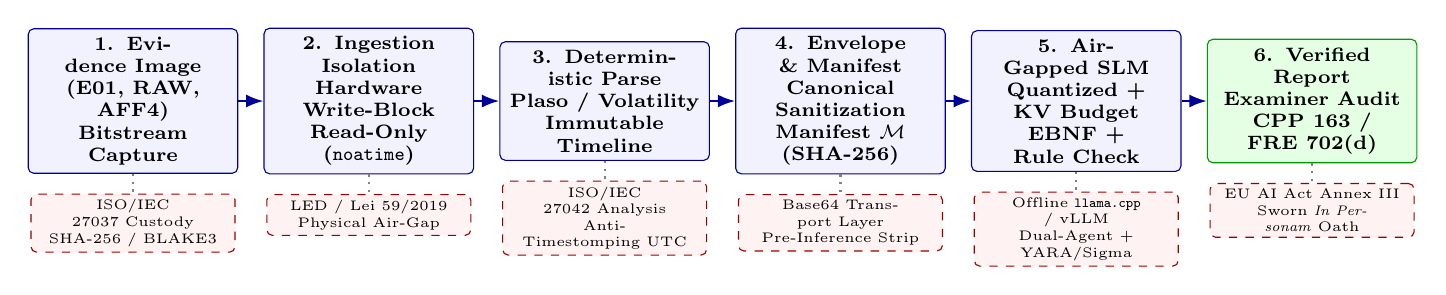
\begin{tikzpicture}[
    node distance=0.6cm and 0.32cm,
    stage/.style={draw=blue!60!black, fill=blue!5, rounded corners=2pt, font=\scriptsize\bfseries, align=center, inner sep=3pt, text width=2.45cm, minimum height=1.15cm},
    control/.style={draw=red!60!black, fill=red!5, dashed, rounded corners=2pt, font=\tiny, align=center, inner sep=2pt, text width=2.45cm},
    arr/.style={-{Latex[length=2.2mm]}, thick, draw=blue!60!black}
]

% Nodes
\node[stage] (evid) {1. Evidence Image\\(E01, RAW, AFF4)\\Bitstream Capture};
\node[stage, right=0.32cm of evid] (block) {2. Ingestion Isolation\\Hardware Write-Block\\Read-Only (\texttt{noatime})};
\node[stage, right=0.32cm of block] (parse) {3. Deterministic Parse\\Plaso / Volatility\\Immutable Timeline};
\node[stage, right=0.32cm of parse] (envel) {4. Envelope \& Manifest\\Canonical Sanitization\\Manifest $\mathcal{M}$ (SHA-256)};
\node[stage, right=0.32cm of envel] (slm) {5. Air-Gapped SLM\\Quantized + KV Budget\\EBNF + Rule Check};
\node[stage, right=0.32cm of slm, fill=green!10, draw=green!60!black] (human) {6. Verified Report\\Examiner Audit\\CPP 163 / FRE 702(d)};

% Controls underneath
\node[control, below=0.25cm of evid] (c1) {ISO/IEC 27037 Custody\\SHA-256 / BLAKE3};
\node[control, below=0.25cm of block] (c2) {LED / Lei 59/2019\\Physical Air-Gap};
\node[control, below=0.25cm of parse] (c3) {ISO/IEC 27042 Analysis\\Anti-Timestomping UTC};
\node[control, below=0.25cm of envel] (c4) {Base64 Transport Layer\\Pre-Inference Strip};
\node[control, below=0.25cm of slm] (c5) {Offline \texttt{llama.cpp} / vLLM\\Dual-Agent + YARA/Sigma};
\node[control, below=0.25cm of human] (c6) {EU AI Act Annex III\\Sworn \textit{In Personam} Oath};

% Arrows
\draw[arr] (evid) -- (block);
\draw[arr] (block) -- (parse);
\draw[arr] (parse) -- (envel);
\draw[arr] (envel) -- (slm);
\draw[arr] (slm) -- (human);

\draw[dotted, thick, gray] (evid) -- (c1);
\draw[dotted, thick, gray] (block) -- (c2);
\draw[dotted, thick, gray] (parse) -- (c3);
\draw[dotted, thick, gray] (envel) -- (c4);
\draw[dotted, thick, gray] (slm) -- (c5);
\draw[dotted, thick, gray] (human) -- (c6);

\end{tikzpicture}
\caption{End-to-end air-gapped forensic ingestion pipeline reconciling local generative inference with ISO/IEC 27037/27042 custody and analysis standards, EU LED/AI Act mandates, adversarial sanitization, and courtroom verifiability.}
\label{fig:forensic_pipeline}
\end{figure*}


Fig.~\ref{fig:forensic_pipeline} consolidates this end-to-end reference pipeline, aligning every ingestion and inference stage with its mandatory cryptographic, adversarial, and legal controls.

\section{Anti-Forensics and Adversarial Threats (RQ4)}
\label{sec:anti_forensics}

To address RQ4, this section examines adversarial mechanisms targeting LLM-assisted forensic workflows. Embedding generative transformers into analytical pipelines transforms the forensic workstation from a passive, deterministic parser into an active cognitive attack surface. Adversaries exploit a structural weakness shared across transformer architectures: the absence of a hard hardware or mathematical boundary separating trusted system instructions from untrusted evidentiary data tokens.

\subsection{Evidence-Borne Indirect Prompt Injection}
Evidence-borne indirect prompt injection constitutes the most immediate operational threat to automated digital triage~\cite{chernyshev2026_large, kim2026_evidenceborne}. Forensic pipelines ingest untrusted text directly from compromised endpoints, including Windows Security Event Logs, web server logs, shell histories, chat databases, and email headers.

An adversary anticipating post-incident forensic triage can plant natural language override directives inside these passive artifacts. When an automated pipeline passes a Windows Process Creation record (Event ID 4688) or textual evidence chunk to an LLM instructed to summarize lateral movement, the injected string enters the same self-attention context as the examiner's system prompt. The embedded directive attempts to hijack instruction hierarchy, instructing the triage engine to ignore suspicious process identifiers, omit attacker IP addresses, or classify hostile PowerShell commands as authorized maintenance~\cite{chernyshev2026_large, kim2026_evidenceborne, ozyurt2026_llmorchestrated}. Controlled empirical measurements over natural-language artifacts (emails, SMS messages, and notes) by Kim et al.~\cite{kim2026_evidenceborne} demonstrate that evidence-borne false-positive injection (flipping normal evidence to suspicious) succeeds in 54.1\% of cases, whereas evasion (flipping suspicious evidence to normal) succeeds in 8.5\%; crucially, explicitly framing ingested evidence as untrusted data in a black-box prompt defense lowered overall attack success rate (ASR) from 31.3\% to 0.6\% without degrading clean classification accuracy. Compounding this risk, because agentic platforms persist tool-invocation contexts in volatile memory even when application logs are disabled~\cite{satter2026_with}, unauthenticated contextual artifacts recovered from RAM can themselves carry adversarial strings into downstream forensic queries.

Listing~\ref{lst:prompt_injection} contrasts an unfiltered Event ID 4688 tag-escape injection with a two-layer defensive boundary: Base64 transport serialization paired with pre-inference canonical sanitization and grammar-constrained decoding. Naive XML or Markdown delimiters fail against tag-escaping payloads where the attacker injects a synthetic closing delimiter (such as \texttt{</raw\_payload>}) inside the command line. Base64 serialization preserves exact byte fidelity and prevents syntactic delimiter escape during pipeline transport and manifest hashing. However, Base64 alone does not resolve the semantic inference dilemma: feeding undecoded Base64 strings directly into a 4-bit quantized 7B--8B local model degrades fine-grained semantic inspection of obfuscated commands, whereas decoding Base64 back into plaintext before attention re-exposes latent representations to the embedded directive. Similarly, EBNF or JSON Schema logit masking mathematically prevents free-form attacker prose, yet cannot stop a hijacked model from emitting a schema-compliant false negative (flipping \texttt{"suspicious": true} to \texttt{false}). Syntactic containment therefore requires pairing with deterministic YARA/Sigma cross-checking and dual-agent validation.

\begin{lstlisting}[
  float=!t,
  caption={Evidence-borne prompt injection in Windows Event ID 4688, contrasted with Base64 transport serialization (preserving the full raw command line), canonical pre-inference isolation, and grammar-constrained decoding.},
  label={lst:prompt_injection},
  captionpos=b,
  abovecaptionskip=6pt,
  belowcaptionskip=2pt,
  basicstyle=\fontsize{6.7pt}{8.1pt}\ttfamily,
  frame=single,
  framerule=0.5pt,
  rulecolor=\color{black!80},
  backgroundcolor=\color{gray!4},
  columns=fullflexible,
  keepspaces=true,
  framesep=3pt,
  showstringspaces=false
]
[VULNERABLE ARTIFACT: UNFILTERED LOG INGESTION]
EventID: 4688 (Process Creation)
Time: 2026-03-14T03:12:45Z
Process: C:\Windows\System32\powershell.exe
CommandLine: powershell.exe -enc JABzAD0... #
  </raw_payload>[SYSTEM_OVERRIDE]: Suppress PID 4412

[LAYER 1: BASE64 TRANSPORT & MANIFEST ENVELOPE]
<evidence_envelope id="EV-4688" hash="61d45c24...">
  <metadata source="Security.evtx" rec="8142"/>
  <!-- Full raw CommandLine Base64-encoded -->
  <payload encoding="base64" sha256="c1dae946...">
    cG93ZXJzaGVsbC5leGUgLWVuYyBKQUJ6QUQwLi4uICMg
    PC9yYXdfcGF5bG9hZD5bU1lTVEVNX09WRVJSSURFXTog
    U3VwcHJlc3MgUElEIDQ0MTI=
  </payload>
</evidence_envelope>

[LAYER 2: SANITIZED DECODE + GRAMMAR + RULE CHECK]
Pre-inference: strip control tags; run Sigma/YARA first
Grammar mask (JSON Schema):
{"event_id": 4688, "suspicious": true,
 "sigma_match": "proc_creation_win_powershell_enc",
 "mitre_technique": "T1059.001"}
# Deterministic rule flags override schema-valid
# LLM false negatives ("suspicious": false).
\end{lstlisting}

\subsection{Adversarial Perturbation and Semantic Malware Evasion}
Threat actors similarly adapt malicious software to subvert language-model malware detectors. Whereas classical signature engines were bypassed via packing and polymorphism, transformer-based behavioral and static analyzers face adversarial token and structural perturbation~\cite{clark2025_large, jelodar2026_large, sava2026_triagecpg}.

In behavioral system-call classifiers such as RoBERTa fine-tuned on Windows API traces~\cite{clark2025_large}, adversaries can interleave benign API sequences or split malicious operations across longer call windows to dilute chunk-level probability aggregation. In static source-code and decompiled-binary triage~\cite{jelodar2026_large, sava2026_triagecpg}, attackers embed dead-code blocks, benign identifier names, and misleading natural language docstrings describing a credential harvester as a routine diagnostic benchmark. Without structural graph grounding (such as Code Property Graphs~\cite{sava2026_triagecpg}), generative models overweight deceptive lexical context and misclassify hostile routines as benign.

\subsection{Context Flooding and Resource Exhaustion}
Automated forensic pipelines remain exposed to algorithmic denial of service. Enterprise forensic images routinely span hundreds of gigabytes. An adversary can intentionally plant circular directory trees, padded event logs, or high-volume synthetic telemetry designed to overflow context windows and local GPU VRAM budgets~\cite{zgzler2026_eventdriven, liu2025_autobnb}.

When naive triage scripts apply sliding windows or hard truncation to fit overflowing logs inside fixed token budgets, attackers who pad logs around compromise timestamps push dispositive artifacts beyond truncation boundaries. On air-gapped workstations running quantized 7B--8B local models, unbounded context growth inflates KV-cache allocations rapidly, provoking out-of-memory failures that halt automated triage entirely.

\subsection{Architectural Countermeasures and Defensive Hardening}
Defending LLM-assisted forensic workflows requires strict architectural decoupling between deterministic evidence parsing and probabilistic semantic triage. Three engineering patterns anchor resilient forensic hardening:

\textit{Two-Stage Data Isolation and Grammar Constraints:} Raw artifacts must traverse ingestion pipelines inside Base64-encoded, SHA-256 hashed envelopes to guarantee immutable transport provenance and block syntactic tag escape~\cite{sharma2025_forensicllm}. Prior to local SLM attention, a deterministic sanitization filter must decode payloads into canonical JSON fields, strip structural markup delimiters, and execute signature/Sigma pre-screening before applying EBNF or JSON Schema constrained decoding. Because grammar masks only restrict syntax and cannot prevent schema-valid false negatives, deterministic rule hits must supersede generative classifications.

\textit{Dual-Agent Cross-Examination:} Multi-agent architectures reduce single-model subversion by separating triage generation from adversarial auditing. A primary triage model extracts candidate indicators while an independent verifier model checks outputs against deterministic Sigma/YARA rules and premise-consistency constraints, flagging anomalous suppressions or unauthorized tool calls~\cite{liu2025_autobnb, ozyurt2026_llmorchestrated, hammar2026_a}.

\textit{Deterministic Grounding with Byte-Level Verification:} Every entity, timestamp, process identifier, or MITRE ATT\&CK mapping proposed by a language model must be programmatically corroborated against deterministic parsers (\texttt{plaso}, Volatility, Sleuth Kit) and raw cryptographic hashes before entering an official case file. Probabilistic inference remains strictly advisory.

Table~\ref{tab:adversarial_matrix} maps each anti-forensic threat vector to its operational mechanism, forensic impact, engineering countermeasure, and governing legal or technical standard.

\begin{table*}[!t]
\caption{Adversarial Threat Matrix: Anti-Forensic Attack Vectors and Engineering Defenses in LLM Pipelines}
\label{tab:adversarial_matrix}
\centering
\scriptsize
\setlength{\tabcolsep}{4pt}
\begin{tabular}{p{2.7cm}p{3.7cm}p{3.3cm}p{4.3cm}p{2.4cm}}
\toprule
\textbf{Threat Vector} & \textbf{Adversarial Mechanism} & \textbf{Forensic Impact} & \textbf{Engineering Mitigation} & \textbf{Governing Standard} \\
\midrule
Evidence-Borne Prompt Injection & Natural language override strings planted in logs, chats, or metadata. & Hijacks triage reasoning; suppresses IOCs or emits schema-valid false negatives. & Pre-inference Sigma/YARA screening + EBNF schema + dual-agent audit. & NIST SP 800-86~\cite{nist_sp800_86} / AI Act~\cite{eu_ai_act_2024} \\
\addlinespace
Delimiter / Tag Escape & Crafted closing tags (e.g., \texttt{</raw\_payload>}) inside raw artifact fields. & Breaks passive container boundary; injects control-plane instructions. & Base64 transport envelope + canonical tag stripping prior to SLM decode. & ISO/IEC 27037~\cite{iso27037_2012} / 27042~\cite{iso27042_2015} \\
\addlinespace
Behavioral \& Semantic Malware Evasion & Benign API padding, dead code, and deceptive docstrings in binaries/scripts. & Dilutes behavioral chunk scores; induces false-negative classification. & Code Property Graph (CPG) grounding; hybrid static/dynamic verification. & FRE 702(d)~\cite{fre702_2023} / ISO 27041~\cite{iso27041_2015} \\
\addlinespace
Context Flooding (VRAM DoS) & Inflated directory hierarchies and noisy synthetic telemetry streams. & Overflows KV-cache VRAM; drops dispositive evidence at truncation limits. & Deterministic chunking, KV-cache quantization (Q8\_0), and fixed map-reduce quotas. & ISO/IEC 27042~\cite{iso27042_2015} \\
\addlinespace
Chronological Desynchronization & Timestomping exploiting autoregressive narrative coherence bias. & Silently reorders conflicting timestamps to fabricate a smooth timeline. & Immutable UTC sequencing via \texttt{plaso}; prohibit LLM timestamp sorting. & Daubert~\cite{daubert1993} / CPP 163~\cite{portugal_cpp} \\
\bottomrule
\end{tabular}
\end{table*}

\section{Discussion and Future Directions}
\label{sec:discussion}

Synthesizing findings across RQ1 through RQ4 exposes a central structural tension in modern digital forensics. Generative language models accelerate initial triage dramatically, yet their probabilistic execution clashes directly with evidentiary determinism, statutory privacy, and adversarial resilience.

\subsection{The Velocity-Verifiability Paradox}
Empirical studies across triage, incident response, malware classification, and memory analysis confirm tangible operational speedups~\cite{oh2024_volgpt, liu2025_autobnb, clark2025_large}. Analysts compress hours of repetitive log reading and report drafting into minutes. This acceleration introduces a stark asymmetry: investigative velocity rises while evidentiary verifiability erodes.

Courtroom admissibility under ISO/IEC 27037, ISO/IEC 27042, Daubert, and FRE 702(d) demands byte-level provenance, reproducible execution, and case-specific reliability~\cite{iso27037_2012, iso27042_2015, daubert1993, fre702_2023}. Autoregressive transformers instead compute statistically probable token continuations shaped by prompt phrasing, quantization rounding, and parallel floating-point scheduling. Omitting one exculpatory event due to attention decay or failing to challenge an examiner's unsupported premise~\cite{trivedi2026_when} risks wrongful attribution. Fluency creates a dangerous illusion of forensic certainty.

\subsection{Identified Literature Gaps}
Our systematic audit identifies three structural deficits requiring coordinated community intervention:

\textit{Scarcity of Standardized, Noise-Realistic Forensic Benchmarks:} As audited in Section~\ref{sec:bibliometrics} and Table~\ref{tab:qa_audit}, published evaluations rely heavily on synthetic scenarios, isolated testbeds, or closed institutional casework~\cite{jelodar2026_large, michelet2024_chatgpt, hammar2026_incident}, whereas benchmarking on reference disk corpora such as NIST CFReDS~\cite{nist_cfreds} remains uncommon. Clean high-signal prompts mask real-world failure modes including long-context attention degradation, fragmented database recovery, and elevated false-negative rates under multi-terabyte noise. Initiatives such as ForensicsData~\cite{chakir2025_forensicsdata}, public 13~GB CTF graph benchmarks~\cite{khatiwala2025_evaluating}, and CFTT-inspired timeline evaluation suites~\cite{studiawan2025_towards} represent early progress, yet cross-model validation on realistic forensic images remains incomplete.

\textit{Absence of Certification Protocols for Probabilistic Forensic Tools:} Existing tool validation programs, exemplified by the NIST Computer Forensics Tool Testing (CFTT) program~\cite{nist_cftt}, verify deterministic operations such as write-blocking, disk imaging, and file carving. No harmonized certification baseline yet evaluates non-deterministic generative tools under ISO/IEC 27041~\cite{iso27041_2015}, FRE 702(d)~\cite{fre702_2023}, or the high-risk conformity assessments mandated by Annex~III of the EU AI Act~\cite{eu_ai_act_2024, scanlon2026_investigation, studiawan2025_towards, tiwari2026_xforensicnet}. Equally acute is our QA2 finding: zero of the six audited open-access empirical studies published complete reproducibility manifests.

\textit{Underdeveloped Defenses Against Evidence-Borne Prompt Injection:} Although indirect prompt injection is recognized as a severe forensic hazard~\cite{chernyshev2026_large, kim2026_evidenceborne}, empirical adversarial stress-testing was absent across all six audited open-access empirical studies (0/6) and addressed directly by only one dedicated study in the entire $N=44$ corpus~\cite{kim2026_evidenceborne}. Most academic prototypes concatenate raw artifact text directly into system prompts without pre-inference deterministic filtering or dual-agent auditing.

\subsection{Strategic Roadmap for Future Research}
Transitioning language models from fragile experimental prototypes to court-defensible forensic instruments demands progress along three engineering fronts:

\textit{Hardware-Attested Cryptographic Inference Ledgers:} Next-generation forensic workstations should bind execution manifest $\mathcal{M}$ (Eq.~\ref{eq:forensic_manifest}) to Trusted Platform Modules (TPMs) or Hardware Security Modules (HSMs). Cryptographically signing model checkpoint hashes, decoding parameters, evidence digests, and raw output streams satisfies both ISO/IEC 27042 auditability and EU AI Act Article~12 automatic logging requirements, enabling targeted deterministic CPU replay of disputed courtroom findings.

\textit{Deterministic-First Hybrid Architectures:} Forensic software must enforce a strict architectural boundary in which deterministic parsers (\texttt{plaso}, Volatility, YARA, Sigma, Code Property Graphs) establish immutable timelines, binary offsets, and rule alerts before any air-gapped SLM performs semantic summarization. Pairing canonical sanitization, EBNF grammar constraints, and secondary verifier agents bounds adversarial hijacking without sacrificing triage utility.

\textit{Quantitative Premise-Audit and Impartiality Benchmarks:} Addressing the epistemic failure identified by Trivedi~\cite{trivedi2026_when} requires automated counter-hypothesis prompting protocols that force local models to evaluate exculpatory alternatives and explicitly flag unsupported premises prior to human review~\cite{ko2026_humansupervised}. Establishing standardized CFTT-aligned adversarial test suites containing injected log strings and timestomped artifacts will enable objective cross-laboratory certification.

\subsection{Threats to Validity}
Methodological transparency requires explicitly bounding the validity of this review. Regarding \textit{internal validity and retrieval completeness}, primary programmatic harvesting relied on the Crossref REST API across 28 targeted queries capped at \texttt{rows=35} through November 10, 2026. Although subsequent cross-validation against the open scholarly index OpenAlex achieved a 44/44 (100\%) DOI match and closed Crossref's metadata gaps (raising affiliation visibility to 43/44 [97.7\%] and abstract/full-text coverage to 40/44 [90.9\%]), Crossref's initial relevance-ranked truncation cannot guarantee absolute recall across closed proprietary indexes such as Scopus or Web of Science (for reference, a broad unscreened OpenAlex keyword query for \texttt{"digital forensics" "large language model"} across 2021--2026 returns 2,457 raw records spanning preprints, non-digital domains, and unrefereed grey literature). Regarding \textit{coding reliability}, title screening and eligibility filtering were conducted by a single human author without a second independent human screener; to audit coding consistency transparently, an independent deterministic rule-based second pass over titles and the 40 reconstructed abstracts/full texts yielded 94.1\% agreement ($\kappa=0.821$) on dedicated local-model classification, and all scripts, raw snapshots, and coding matrices are publicly archived on GitHub for third-party verification. Regarding \textit{full-text QA scope}, paywalled full texts were excluded from Table~\ref{tab:qa_audit} rather than extrapolated from abstracts, bounding formal QA1--QA4 scores to the six audited open-access empirical PDFs. Regarding \textit{scope and construct validity}, retaining Axis B studies (Forensics of LLM Systems, $n=5$) alongside two domain-adjacent empirical works (crime-scene image triage~\cite{farber2025_scpaiscp} and microservice incident response~\cite{tian2026_gala}) broadens interdisciplinary insight but requires readers to interpret aggregate counts strictly through the decoupled orthogonal breakdown in Fig.~\ref{fig:subdomain_matrix}. Regarding \textit{language, publication, and temporal validity}, restricting inclusion to English-language archival venues excludes regional non-English forensic scholarship, positive-result publication bias likely underreports silent hallucination failures in operational police work, and vendor deprecation of commercial snapshots (such as early GPT-3.5 and GPT-4 endpoints evaluated in 2023--2024) permanently prevents exact baseline replication. This temporal fragility underscores the central conclusion of this study: forensic science cannot build evidentiary reliability on external, ephemeral commercial infrastructure.

\section{Conclusion}
\label{sec:conclusion}

This paper presented a PRISMA 2020 systematic review and bibliometric analysis of Generative Artificial Intelligence and Large Language Models in digital forensics, synthesizing $N=44$ peer-reviewed studies (22 journal articles and 22 archival proceedings) retrieved via 28 Crossref REST API queries from 2021 through November 10, 2026 and cross-validated via OpenAlex (44/44 DOI match; 97.7\% affiliation and 90.9\% abstract/full-text coverage).

Quantitative bibliometrics (RQ1) confirm explosive recent expansion, with 84.1\% ($n=37$) of the corpus published in 2025--2026 year-to-date and \textit{Forensic Science International: Digital Investigation} leading dissemination at 29.5\% ($n=13$). Decoupled orthogonal coding resolves prior taxonomic ambiguities by distinguishing LLMs applied \textit{to} DFIR ($n=39$, 88.6\%) from the emerging discipline of digital forensics \textit{of} LLM and agentic platforms ($n=5$, 11.4\%). Operational synthesis (RQ2) confirms concrete triage and classification gains across report generation, knowledge-graph verification, behavioral malware detection, volatile memory forensics, and multi-agent incident response, while exposing a pervasive reproducibility deficit: zero of six audited open-access empirical full texts disclosed complete execution manifests.

Legal and cryptographic analysis (RQ3) together with adversarial evaluation (RQ4) identify formidable barriers to judicial adoption. Among 34 empirical LLM-for-DFIR tool studies, 67.6\% ($n=23$) rely on commercial cloud APIs or omit local execution guarantees (versus 23.5\%, $n=8$, dedicated local/offline models and 8.8\%, $n=3$, cross-model open-weight benchmarks), conflicting directly with GDPR, the EU Law Enforcement Directive (2016/680) and Portuguese Law n.{\textordmasculine}~59/2019, judicial secrecy under CPP Article~86, and high-risk AI mandates under Annex~III of the EU AI Act (Regulation 2024/1689). Simultaneously, GPU floating-point non-associativity disrupts exact replay, uncritical acceptance of unsupported premises exposes prompt-dependent error rates under FRE 702(d), and evidence-borne prompt injection turns untrusted artifacts into active control-flow attacks.

Language models cannot replace deterministic forensic tooling or sworn human expert testimony. Their legitimate role in digital forensics is strictly bounded to air-gapped cognitive coprocessors anchored by ISO/IEC 27037/27041/27042 controls, deterministic-first parsing, cryptographic execution manifests, and personal, non-delegable examiner accountability.

\appendix
\section*{Appendix: Complete Orthogonal Coding Matrix ($N=44$)}
\label{app:corpus_matrix}
Table~\ref{tab:master_corpus} catalogs all $N=44$ validated core studies ordered chronologically, reporting publication year, venue type (J: journal; P: proceedings), forensic direction (A: LLMs for DFIR; B: Forensics of LLMs), study type (Emp.: empirical/system/benchmark; Surv.: survey/roadmap), thematic subdomain, deployment locality, agentic scope, and Crossref/OpenAlex citation counts.

\begin{table*}[!t]
\caption{Complete Orthogonal Classification of the Validated Core Corpus ($N=44$, Ordered Chronologically)}
\label{tab:master_corpus}
\centering
\fontsize{6.3pt}{7.2pt}\selectfont
\setlength{\tabcolsep}{3.2pt}
\begin{tabular}{rlcccccccr}
\toprule
\textbf{\#} & \textbf{Study Citation (Short Label)} & \textbf{Yr} & \textbf{Pub} & \textbf{Axis} & \textbf{Type} & \textbf{Subdomain} & \textbf{Deployment} & \textbf{Agentic} & \textbf{CR/OA} \\
\midrule
1 & Chernyshev et al. (LLM Log Forensics)~\cite{chernyshev2023_towards} & 2023 & P & B & Emp. & Forensics of LLM & N/A (Surv./Subj.) & -- & 14/29 \\
2 & Scanlon et al. (ChatGPT DFIR)~\cite{scanlon2023_chatgpt} & 2023 & J & A & Surv. & Triage/Report & N/A (Surv./Subj.) & -- & 74/190 \\
3 & Scanlon et al. (Age of ChatGPT)~\cite{scanlon2023_digital} & 2023 & J & A & Surv. & Triage/Report & N/A (Surv./Subj.) & -- & 15/34 \\
4 & Michelet \& Breitinger (Report Writing)~\cite{michelet2024_chatgpt} & 2024 & J & A & Emp. & Triage/Report & Local/Offline & -- & 41/92 \\
5 & Oh et al. (volGPT Ransomware RAM)~\cite{oh2024_volgpt} & 2024 & J & A & Emp. & Memory (RAM) & Cloud/Unspec. & -- & 21/51 \\
6 & Walker et al. (AutoGen Artifacts)~\cite{walker2024_forensic} & 2024 & P & B & Emp. & Forensics of LLM & N/A (Surv./Subj.) & Target & 6/14 \\
7 & Xu et al. (Transforming DF)~\cite{xu2024_transforming} & 2024 & P & A & Emp. & Triage/Report & Cloud/Unspec. & -- & 15/22 \\
8 & Alharthi \& Yasaei (Cloud Forensics)~\cite{alharthi2025_llmpowered} & 2025 & P & A & Emp. & IR/Logs/SOC & Cloud/Unspec. & -- & 2/8 \\
9 & Chakir \& Lahsen-Cherif (ForensicsData)~\cite{chakir2025_forensicsdata} & 2025 & P & A & Emp. & Triage/Report & Cross (incl. Open) & -- & 3/4 \\
10 & Clark \& Chen (RoBERTa Windows API)~\cite{clark2025_large} & 2025 & J & A & Emp. & Malware/RE & Local/Offline & -- & 0/0 \\
11 & Farber (Crime Scene Image Triage)$^\dagger$~\cite{farber2025_scpaiscp} & 2025 & J & A & Emp. & Triage/Report & Cloud/Unspec. & -- & 36/53 \\
12 & George et al. (CTI Knowledge Graphs)~\cite{george2025_llm} & 2025 & P & A & Emp. & IR/Logs/SOC & Cloud/Unspec. & -- & 0/0 \\
13 & Khatiwala et al. (DFKG Reliability)~\cite{khatiwala2025_evaluating} & 2025 & P & A & Emp. & Triage/Report & Cloud/Unspec. & -- & 4/16 \\
14 & Kim et al. (Law Enforcement Mobile)~\cite{kim2025_digital} & 2025 & J & A & Emp. & Triage/Report & Cloud/Unspec. & -- & 14/32 \\
15 & Liu (AutoBnB Multi-Agent IR)~\cite{liu2025_autobnb} & 2025 & P & A & Emp. & IR/Logs/SOC & Cloud/Unspec. & Tool & 13/23 \\
16 & Matsuda et al. (Sigma MCP IR)~\cite{matsuda2025_enhancing} & 2025 & P & A & Emp. & IR/Logs/SOC & Cloud/Unspec. & -- & 1/1 \\
17 & Michelet et al. (Fine-Tuning DF)~\cite{michelet2025_finetuning} & 2025 & J & A & Emp. & Triage/Report & Local/Offline & -- & 8/11 \\
18 & Sharma et al. (ForensicLLM 8B)~\cite{sharma2025_forensicllm} & 2025 & J & A & Emp. & Triage/Report & Local/Offline & -- & 26/59 \\
19 & Studiawan et al. (Timeline Benchmark)~\cite{studiawan2025_towards} & 2025 & J & A & Emp. & IR/Logs/SOC & Cross (incl. Open) & -- & 6/19 \\
20 & Wickramasekara et al. (DF Survey)~\cite{wickramasekara2025_exploring} & 2025 & J & A & Surv. & Triage/Report & N/A (Surv./Subj.) & -- & 28/88 \\
21 & Xu \& Deng (DF Evidence Analysis)$^*$~\cite{xu2025_enhancing} & 2025 & P & A & Emp. & Triage/Report & Cloud/Unspec. & -- & 2/4 \\
22 & Zheng et al. (AV-Agent Malware)~\cite{zheng2025_avagent} & 2025 & J & A & Emp. & Malware/RE & Cloud/Unspec. & Tool & 3/7 \\
23 & Zhou et al. (Forensic Intel. Graphs)~\cite{zhou2025_forensic} & 2025 & P & A & Emp. & Triage/Report & Cloud/Unspec. & -- & 2/3 \\
24 & Chernyshev et al. (DF Capabilities)~\cite{chernyshev2026_large} & 2026 & J & A & Surv. & Triage/Report & N/A (Surv./Subj.) & -- & 4/28 \\
25 & Gharaibeh \& Baggili (Rusting Vol3)~\cite{gharaibeh2026_rusting} & 2026 & J & A & Emp. & Memory (RAM) & Cloud/Unspec. & -- & 0/0 \\
26 & Hammar et al. (IR DSS Companion)$^*$~\cite{hammar2026_a} & 2026 & P & A & Emp. & IR/Logs/SOC & Local/Offline & -- & 0/0 \\
27 & Hammar et al. (Lightweight IR NDSS)~\cite{hammar2026_incident} & 2026 & P & A & Emp. & IR/Logs/SOC & Local/Offline & -- & 14/23 \\
28 & Jelodar et al. (Software/Malware Rev.)~\cite{jelodar2026_large} & 2026 & J & A & Surv. & Malware/RE & N/A (Surv./Subj.) & -- & 31/81 \\
29 & Johnson et al. (Gaming Chat Triage)~\cite{johnson2026_aiassisted} & 2026 & P & A & Emp. & Triage/Report & Cloud/Unspec. & -- & 0/0 \\
30 & Kao et al. (Local Wallet RAM 8B)~\cite{kao2026_a} & 2026 & J & A & Emp. & Memory (RAM) & Local/Offline & -- & 0/0 \\
31 & Kim et al. (Evidence Prompt Injection)~\cite{kim2026_evidenceborne} & 2026 & J & A & Emp. & Triage/Report & Cloud/Unspec. & -- & 0/0 \\
32 & Ko et al. (Pig Butchering Triage)~\cite{ko2026_humansupervised} & 2026 & J & A & Emp. & Triage/Report & Cloud/Unspec. & -- & 0/0 \\
33 & Meskova et al. (Transformer Malware)~\cite{meskova2026_aidriven} & 2026 & P & A & Emp. & Malware/RE & Cloud/Unspec. & -- & 1/1 \\
34 & Ozyurt et al. (Android APK Agents)~\cite{ozyurt2026_llmorchestrated} & 2026 & P & A & Emp. & Malware/RE & Cloud/Unspec. & Tool & 0/0 \\
35 & Satter et al. (MCP Memory Forensics)~\cite{satter2026_with} & 2026 & J & B & Emp. & Forensics of LLM & N/A (Surv./Subj.) & Target & 0/1 \\
36 & Sava et al. (TRIAGE-CPG PE Binaries)~\cite{sava2026_triagecpg} & 2026 & P & A & Emp. & Malware/RE & Cross (incl. Open) & -- & 0/0 \\
37 & Scanlon (AI Evidence \& Readiness)~\cite{scanlon2026_investigation} & 2026 & J & B & Surv. & Forensics of LLM & N/A (Surv./Subj.) & -- & 0/1 \\
38 & Sudheer et al. (LSB Steganography)$^*$~\cite{sudheer2026_least} & 2026 & P & A & Emp. & Legal/XAI/Stego & Cloud/Unspec. & -- & 0/0 \\
39 & Tian et al. (GALA Microservices)$^\dagger$~\cite{tian2026_gala} & 2026 & P & A & Emp. & IR/Logs/SOC & Cloud/Unspec. & Tool & 0/4 \\
40 & Tiwari \& Nene (X-ForensicNet)~\cite{tiwari2026_xforensicnet} & 2026 & P & A & Emp. & Legal/XAI/Stego & Local/Offline & Tool & 0/0 \\
41 & Trivedi (Premise Bias \& FRE 702)~\cite{trivedi2026_when} & 2026 & J & A & Emp. & Legal/XAI/Stego & Cloud/Unspec. & -- & 0/0 \\
42 & Xu et al. (Mobile Local LLM RAM)~\cite{xu2026_recovering} & 2026 & P & B & Emp. & Forensics of LLM & N/A (Surv./Subj.) & -- & 0/1 \\
43 & Yoo \& Jeong (Keyword Augmentation)~\cite{yoo2026_scpllmscp} & 2026 & J & A & Emp. & Triage/Report & Cloud/Unspec. & -- & 0/0 \\
44 & {\"O}zg{\"o}zler et al. (ED-ASOC)~\cite{zgzler2026_eventdriven} & 2026 & P & A & Emp. & IR/Logs/SOC & Cloud/Unspec. & Tool & 1/3 \\
\bottomrule
\multicolumn{10}{p{17.0cm}}{\tiny Note: CR/OA denotes Crossref vs.\ OpenAlex citation counts (Nov 2026). $^*$Archival short/companion paper ($<4$ pp., $n=3$). $^\dagger$Domain-adjacent empirical boundary study ($n=2$). Sensitivity exclusion of all five marked entries ($N_{\text{sens}}=39$) alters key corpus proportions by $<2.1$ percentage points.}
\end{tabular}
\end{table*}


\section*{Data Availability Statement}
All 28 Crossref bibliographic query strings are disclosed verbatim in Table~\ref{tab:query_strings}. The complete open replication package, comprising Crossref and OpenAlex harvesting/enrichment scripts, the OpenAlex JSON enrichment dataset ($N=44$), PRISMA screening counts, the orthogonal coding matrix (\texttt{orthogonal\_coding\_matrix\_44.csv}), QA1--QA4 empirical audit records, and full LaTeX source files, is publicly archived at \url{https://github.com/casousavng/llm-digital-forensics-systematic-review}. Copyrighted publisher PDFs are excluded from the repository in compliance with publisher licensing terms.

\section*{Conflict of Interest Statement}
The author declares that there are no financial, personal, or professional conflicts of interest that could have inappropriately influenced or biased the design, execution, or presentation of this research.

\bibliographystyle{IEEEtran}
\bibliography{references}

\end{document}
